%-------------------------------------------------------------------------
%\documentclass[11pt,authoryear]{elsarticle}
\documentclass[authoryear,11pt]{elsarticle}


\setlength{\parskip}{1em}			% espaciar parrafos
\newtheorem{proposition}{Proposition}
\newtheorem{definition}{Definition}
\newtheorem{proof}{Proof}
\newtheorem{corollary}{Corollary}

\usepackage{hyperref}				% enlaces en el pdf
\hypersetup{backref,colorlinks=true}	% colores en vez de cajas en los enlaces
\usepackage{times}              		% la letra
\usepackage{graphicx}           		% para manejar imagenes
\usepackage{subfigure}          		% para manejar subfiguras
\usepackage{tabularx}		   		% para ajustar el ancho de las columnas
\usepackage[margin=2.5cm]{geometry}	% Change margins
\usepackage[table]{xcolor}			% Colores en el cronograma
\usepackage{multirow}				% Cabecera del cronograma
\usepackage{watermark}				% Para la portada
\usepackage{datetime}				% Fecha de creado
\usepackage{pst-tree}				% Para la taxonomía
\usepackage{stackengine}				% Para listar los articulos en el nodo de la taxonomía
\usepackage{algorithm}				% Para el seudocódigo
\usepackage{setspace}				% Para el seudocódigo
\usepackage{amsmath}					% Para el seudocódigo
\usepackage[noend]{algpseudocode}	% Para el seudocódigo
\usepackage{multicol}				% Para el seudocódigo
%\usepackage{algorithmic}


%-------------------------------------------------------------------------
% Configuring Taxonomy
%-------------------------------------------------------------------------
\setstackEOL{\\}
\def\psedge{\ncangles[angleA=-90,angleB=90]}
\psset{levelsep=20mm,treesep=1cm,nodesep=3pt, arrows=->}
\def\PSBL#1{\small\pspicture(7,0.8)\psTextFrame[shadow,
  fillstyle=solid,linecolor=blue,framearc=0.3](0,0)(7,0.8){%
    \shortstack{#1}}\endpspicture}
\def\PSBS#1{\pspicture(3,.7)\psTextFrame[shadow,
  fillstyle=solid,linecolor=blue,framearc=0.3](0,0)(3,0.8){%
    \shortstack{#1}}\endpspicture}

%-------------------------------------------------------------------------
% Referencias a una palabra
%-------------------------------------------------------------------------
\newcommand{\setword}[2]{%
  \phantomsection
  #1\def\@currentlabel{\unexpanded{#1}}\label{#2}%
}


\begin{document}
	
%------Document data---------------------------------------------------------------
\newcommand{\titulo}{Development of fast algorithms\\ for reduct computation}
\newcommand{\nombre}{Vlad\'imir Rodr\'iguez Diez}
\newcommand{\tutorA}{Jos\'e Francisco Mart\'inez Trinidad}
%------Front page------------------------------------------------------------------
\addtolength{\hoffset}{-0.5cm}
\addtolength{\voffset}{-2.0cm}
\addtolength{\oddsidemargin}{3.0cm}
\newpage
\begin{titlepage}
    \thispagestyle{empty}

		\thiswatermark{\centering \put(-70,-720){
\includegraphics[scale=0.9]{titleINAOE.eps}} }
    
    \begin{center}
        \mbox{ }\par
        \vspace{2.5cm}
        {\huge\bfseries\titulo\par}
        %{\Large \textbf{Student:} \nombre \par \textbf{Advisor:} \tutorA \par}
        {\Large \nombre, \tutorA \par}
        \vspace{3cm}
        {\Large Reporte T\'ecnico No. CCC-16-005\\
        %{\Large  PhD Research Proposal\\
		11 de abril de 2016 \par}
        \vspace{5cm}
        {\Large \copyright~ Coordinaci\'on de Ciencias Computacionales\\
        INAOE\par}
       \vspace{2cm}
    \end{center}
    \begin{center}
    		{\Large
        Luis Enrique Erro 1. \\ Sta. Ma. Tonantzintla, \\ 72840, Puebla, M\'exico. \par}
    \end{center}
    


\end{titlepage}

\addtolength{\hoffset}{0.5cm}
\addtolength{\voffset}{2.0cm}
\addtolength{\oddsidemargin}{-3.0cm}  
	
	\title{Development of fast algorithms for reduct computation}
	
	\author{Vlad\'imir Rodr\'iguez Diez}
	\author{Jos\'e Francisco Mart\'inez Trinidad}
	
	\address{Computer Science Department\\National Institute of
	Astrophysics, Optics and Electronics\\
	Luis Enrique Erro \# 1, Santa Mar\'{\i}a Tonantzintla, Puebla,
	72840, M\'{e}xico} 
%	\email{\{vladimir.rodriguez,fmartine\}@inaoep.mx}
	
	
%	\thispagestyle{empty}
	
	\begin{abstract}
		Information systems in Rough Set Theory (RST) are tables of objects described by some attributes. 
		This type of tables are widely used in different pattern recognition problems particularly in 
		supervised classification. RST reducts are minimal subsets of attributes preserving 
		the discernibility capacity of the whole set of attributes. Reducts computation has an exponential
		complexity regarding the number of attributes in the information system. In the literature several
		algorithms for reduct computation have been reported, but their high computational cost makes 
		infeasible their use in large problems. For this reason, in this research we will develop new fast
		algorithms in two directions, the computation of all reducts and the computation of globally 
		shortest reducts. The proposed algorithms will be faster than state of the art algorithms, and hence 
		make the reduct computation viable for larger information systems than it is today. As part of this 
		PhD research proposal, we present some preliminary results, which show that it is possible developing
		faster algorithms for computing reducts.
	\end{abstract}
	
	\begin{keyword}
		Rough Sets\sep Dimensionality Reduction\sep Reduct Computation.
	\end{keyword}

	\maketitle

\pagebreak 
\tableofcontents
\pagebreak 

%-------------------------------------------------------------------------------
% your earth-shattering contribution

\section{Introduction}
  Rough set theory (RST), proposed by Z. Pawlak in 1982 \citep{Pawlak81,Pawlak81-2,Pawlak82,Pawlak91}, 
  is a relatively new mathematical theory 
  to deal with imperfect knowledge, in particular with vague concepts. Into RST, information systems
  are tables of objects described by a set of attributes (columns). 
  When data is collected or recorded, every single aspect (attribute) of the object under study is considered 
  to have a complete representation and to ensure that no potentially useful information is lost.
  As a result, information systems are usually characterized by a large number of attributes,
  degrading the performance of machine learning tools~\citep{Parthalain08}.
  One of the main concepts in RST is the notion of reduct, which is a minimal subset of attributes 
  preserving the required classification capabilities~\citep{Pawlak91}. A new information system using 
  only those features in a reduct, is a reduced representation of the original data that allows obtaining  
  the same classification quality than the original information system. 
  However, the main restriction in practical applications of RST is that computing all reducts of an information 
  system has an exponential complexity~\citep{Skowron92}. Therefore an active research line is the development 
  of fast algorithms for reduct computation.
  
  Several attempts to speed up the reduct computation have been reported. Many of these algorithms are 
  based on some heuristics. The main drawback of this approach is that these algorithms do not necessarily 
  return the complete set of reducts in the information system, and may obtain super-reducts (non minimal subsets). 
  Another way to speed up reduct computation is parallelization~\citep{Strakowski08}. There are also 
  interesting alternatives such as the use of a parallel version of genetic algorithms \citep{Wroblewski98}
  and the transformation of the reduct computation problem to the well known SAT problem~\citep{Jensen14}.
  
  Recently the RST reducts have been related to the typical testors (TT) from the logical combinatorial approach to 
  pattern recognition~\citep{Lazo15}. Testor Theory was created by Yablonskii and Chegis in the middle of fifties 
  of the last century as a tool for analysis of problems connected with control and diagnosis of faults in
  circuits. 
  Testor Theory can be used for feature selection as shown in~\citep{Ruiz08} and~\citep{Martinez01}. Algorithms for
  typical testors computation like~\citep{Ruiz85},~\citep{Santiesteban03},~\citep{Sanchez07} 
  and~\citep{Lias09}, can be applied to reduct computation due to the similarity between these two concepts. 
  Fast implementations of these algorithms; based on cumulative binary operations~\citep{Sanchez10}, genetic 
  algorithms~\citep{Sanchez99} and hardware architectures~\citep{Rojas12}; have been developed to reduce the
  computation time. One strength of our research is that we will be testing, for the first time, these two 
  families of algorithms in the same arena.
     
  Throughout our research we will conduct a comparative study between the most relevant algorithms for reduct 
  computation. Although our main focus will be on algorithms for computing all reducts and globally shortest
  reducts, experiences from heuristics approaches will be considered as well. We will be exploring the relationship 
  between algorithms' performance and the characteristics of the information system. Based on this relationship,
  we will propose fast algorithms for reduct computation. Finally the proposed algorithms 
  will be redesigned and implemented in a hardware fashion in order to improve, even more, their efficiency.  

\section{Basic Concepts}\label{basicConcepts}
  RST is based on the assumption that every object in the universe of discourse is described, through a 
  set of attributes, by some information associated to it. This information constitutes the basis for the
  classification of unseen objects. RST motto is \textit{Let the data speak for themselves} \citep{Tiwari14}.
  
  From the RST point of view, two objects are indistinguishable (indiscernible) if they have an equivalent 
  value for each attribute in their description. Indiscernibility relations arising this way constitute the
  mathematical foundations of RST. 
  Some basic concepts of RST are presented bellow. Although we will be following the explanation 
  in~\citep{Polkowski00}, some modifications in the notation are introduced to provide clarity in the rest 
  of the document.
  
\subsection{Information System}
  The basic representation of data in RST is an \emph{Information System} (IS). An IS is a table with rows
  representing objects while columns specify attributes or features. Formally, an IS is defined as a pair
  $IS=(U,A)$ where $U$ is a finite non-empty set of objects $U=\lbrace x_1,x_2,...,x_n\rbrace$, and $A$ is a 
  finite non-empty set
  of attributes (features, variables). Every attribute in $A$ is a map: $a: U \rightarrow V_a$. The set $V_a$ is
  called the \textit{value set} of $A$. Attributes in $A$ are further divided into condition attributes $C$ and 
  decision attributes $D$ such that $A=C \cup D$ and $C \cap D =\emptyset$. 
  Table~\ref{tab_IS} shows an example IS.
  
  
 \begin{table}[htb]
		\caption{An Information System.} \label{tab_IS}
		\centering
 	\begin{tabular}{c||c|c|c||c}
 			  & $c_1$ & $c_2$ &  $c_3$ & $d$ \\
 		\hline \hline
		$x_1$ &   1   &    3  &  0  &   0   \\
		$x_2$ &   1   &    0  &  0  &   0   \\
		$x_3$ &   3   &    1  &  1  &   1   \\
		$x_4$ &   3   &    3  &  2  &   1   \\
		$x_5$ &   4   &    2  &  3  &   1   \\
		$x_6$ &   4   &    3  &  1  &   0   \\
		$x_7$ &   4   &    2  &  5  &   1   \\
 	\end{tabular}             
 \end{table}
 
   
  \textit{Decision attributes} determine to which class the object belongs. In the IS of
  table~\ref{tab_IS}, $d$ is the decision attribute. 
  %For this example $V_d = \lbrace 0,1 \rbrace$; hence 
  This is a two-class system. \textit{Condition attributes} do not absolutely determine the class but help 
  to decide to which class an object belongs to. In supervised classification, condition attributes are the 
  only information available for classifying new objects; while, decision attributes are only 
  available for objects in the training set. An IS with distinguished decision and condition attributes is 
  called a decision table. In table~\ref{tab_IS}, $c_1$, $c_2$ and $c_3$ are condition attributes.
 
%\subsection{Indiscernibility Relations}
%  For an object $x \in U$, the information about $x$ with respect to a set $B \subseteq A$ may be defined as
%  \textit{the B-information set} 
%  
%  \begin{equation}
%  	Inf_B(x)=\lbrace (a,a(x)):a \in B \rbrace
%  \end{equation}  
%  
%  of $x$.
%  
%  \emph{Indiscernibility relation} of $B$ is defined as follows:
%  
%  \begin{equation}
%  	(x,y) \in IND_B \Longleftrightarrow Inf_B(x)=Inf_B(y)
%  \end{equation} 
%  
%  Equivalent classes $[x]_B$ of the relation $IND_B$ represent therefore elementary (atomic) portions
%  of knowledge represented by the subsystem $IS_B=(U,B)$.
%  
%  For a \textit{concept} (set of objects), $X \subseteq U$, we say that $X$ is \textit{B-exact} if and 
%  only if
%  	
%  \begin{equation}
%  	X=\cup_{i=1}^{k} [x_i]_B
%  \end{equation} 
%  
%  for some $x_1, x_2,...,x_k \in U$ i.e. where $X$ is the union of some \textit{B-indiscernibility} classes.
%  
%  For example, in table~\ref{tab_IS} the three possible subset of conditional attributes are 
%  $\lbrace c_1 \rbrace$, $\lbrace c_2 \rbrace$ and $\lbrace c_1, c_2 \rbrace$. The indiscernibility relation 
%  for these sets defines three partitions of the universe:
%  
%  $$\begin{array}{lcc}
%  IND_{\lbrace c_1 \rbrace} &=& \lbrace \lbrace x_1, x_2 \rbrace, 
%  								\lbrace x_3, x_4 \rbrace, 
%  								\lbrace x_5, x_6, x_7 \rbrace \rbrace \\
%  IND_{\lbrace c_2 \rbrace} &=& \lbrace \lbrace x_1, x_4, x_6 \rbrace, 
%  								\lbrace x_2 \rbrace, 
%  								\lbrace x_3 \rbrace,
%  								\lbrace x_5, x_7 \rbrace \rbrace \\
%  IND_{\lbrace c_1, c_2 \rbrace} &=& \lbrace \lbrace x_1 \rbrace, 
%  									\lbrace x_2 \rbrace, 
%  									\lbrace x_3 \rbrace,
%  									\lbrace x_4 \rbrace,
%  									\lbrace x_5, x_7 \rbrace,
%  									\lbrace x_6 \rbrace \rbrace 
%  \end{array}$$
%
%\subsection{Concept Approximations}
%  RST capability of handling non-exact (rough) concepts arises from the approximation of a rough concept 
%  by means of two crisp concepts: the \textit{lower} and the \textit{upper approximations of} $X$. 
%  Denoted by $\underline{B}X$ and $\overline{B}X$, respectively as follows:
%  
%  \begin{equation}
%  	\begin{array}{lcc}
%  	\underline{B}X &=& \lbrace x \in U : [x]_B \subseteq X \rbrace\\
%  	\overline{B}X  &=& \lbrace x:[x]_B \cap X \neq \emptyset \rbrace
%  	\end{array}
%  \end{equation}
%  
%  We would say that objects in $\underline{B}X$ can be certainly classified as elements of $X$ on the 
%  basis of knowledge in $IS_B$, while objects in $\overline{B}X$ can only be possibly classified as 
%  elements of $X$ on the basis of knowledge in $IS_B$. In other words, $\underline{B}X$ is 
%  composed by those objects in $X$ having no indiscernible objects outside $X$. $\overline{B}X$ on the 
%  other hand, is composed by all objects in $X$ plus all objects outside $X$ having an indiscernible 
%  object in $X$.
%  
%  The set 
%  
%  \begin{equation}
%  	BN_B(X)=\overline{B}X-\underline{B}X
%  \end{equation}
%  
%  is called the \textit{B-boundary region of X} and it contains the objects which neither are certainly 
%  members of $X$ nor they are certainly member of $U-X$. The presence of a non-empty boundary region
%  indicates that the concept in question is rough (\textit{B-rough}).
%  
%  From the previous example we can see that e.g. concept $X=\lbrace x_1,x_2,x_3 \rbrace$ is rough for the 
%  three attributes sets while e.g. the concept $Y=\lbrace x_1,x_2 \rbrace$ is both $\lbrace c_2 \rbrace$-
%  and $\lbrace c_1, c_2 \rbrace$-exact. Notice that
%  
%  $$\begin{array}{lcc}
%  \underline{c_1}X &=& \emptyset\\
%  \overline{c_1}X  &=& \lbrace x_1,x_2,x_3,x_4,x_6 \rbrace\\
%  \underline{c_2}X &=& \lbrace x_1,x_2 \rbrace
%  \end{array}$$
  
\subsection{Positive Region}\label{subsect_Pos}
  Decision attributes induce a partition of the universe $U$ into equivalence classes 
  (\textit{decision classes}). Since we will be trying to associate a decision class to an object, 
  based on the attributes belonging to $B \subseteq C$, we are interested in those 
  $B-classes$ (classes induced by $B$) which correspond to classes induced by $d$. 
  This idea leads to the notion of the  \textit{positive region of the decision}. The set $POS_B(d)$, 
  called the \textit{B-positive region of d}, is defined as the set of all objects in $U$ such 
  that all their indistinguishable objects (under the knowledge in $B$) belong to its same class induced 
  by $d$.
  
  Taking for example the IS in table~\ref{tab_IS}, we can see that
  
  $$\begin{array}{lcc}
  POS_{\lbrace c_1 \rbrace}(d)     &=& \lbrace x_1,x_2,x_3,x_4 \rbrace\\
  POS_{\lbrace c_2 \rbrace}(d)     &=& \lbrace x_2,x_3,x_5,x_7 \rbrace\\
  POS_{\lbrace c_1, c_2 \rbrace}(d)&=& U
  \end{array}$$
 
\subsection{Reducts and Core}\label{def_reduct}
  Given an information system $IS=(U,A)$ with condition attribute set $C$ and decision attribute set
  $D$ such that $A=C \cup D$ and $C \cap D =\emptyset$. A subset $B \subseteq C$ is a \textit{reduct} 
  of $IS$ relative to $D$ if
  \begin{enumerate}
  	\item $POS_B(D)=POS_C(D)$. \label{cond_1}
  	\item $B$ is a minimal subset (with respect to inclusion) satisfying condition~\ref{cond_1}.\label{cond_2}
  \end{enumerate}

  We call any subset $B \subseteq C$ satisfying condition~\ref{cond_1} a super-reduct whether it satisfies
  condition~\ref{cond_2} or not.
  
  The intersection of all reducts of an IS is called the \textit{core}, the attributes that cannot be
  eliminated without reducing the classification accuracy.
  
\subsection{Discernibility Matrix and Discernibility Function}
  The discernibility knowledge of the information system is commonly stored in a symmetric $|U| \times |U|$
  matrix called the \textit{discernibility matrix}. Each element $m_{ij}$ in the discernibility matrix 
  $M_{IS}$ is defined as   
  \begin{equation}
  	m_{ij}=\left\lbrace\begin{array}{cl}
  			\lbrace c \in C: c(x_i) \neq c(x_j) \rbrace & \mathrm{for~~}D(x_i) \neq D(x_j)\\
  			\emptyset 								   & \mathrm{otherwise} 
  	\end{array}\right.
  \end{equation}  
  Here, $c(x_i)$ stands for the value of the condition attribute $c$ in the object (row) $x_i$, and 
  $$D(x_i) \neq D(x_j) \Rightarrow \exists d \in D~ |~ d(x_i) \neq d(x_j)$$ 
  where $d(x_i)$ stands for the value  of the decision attribute $d$ in the object $x_i$.
  
  Table~\ref{tab_DM} shows the discernibility matrix for the IS in table~\ref{tab_IS} as a lower triangular 
  matrix ($\emptyset$'s are omitted for clarity).
  
   \begin{table}[htb]
		\caption{Discernibility Matrix Example.} \label{tab_DM}
		\centering
 	\begin{tabular}{c|ccccccc}
 		$x \in U$ & 1 & 2 &  3 & 4 & 5 &  6 & 7\\
 		\hline
		1 &&&&&&&\\
		2 &&&&&&&\\
		3 & $\lbrace c_1,c_2,c_3\rbrace$ & $\lbrace c_1,c_2,c_3\rbrace$ &&&&&\\
		4 & $\lbrace c_1,c_3\rbrace$ & $\lbrace c_1,c_2,c_3\rbrace$ &&&&&\\
		5 & $\lbrace c_1,c_2,c_3\rbrace$ & $\lbrace c_1,c_2,c_3\rbrace$ &&&&&\\
		6 &&& $\lbrace c_1,c_2\rbrace$ & $\lbrace c_1,c_3\rbrace$ & $\lbrace c_2,c_3\rbrace$ &&\\
		7 & $\lbrace c_1,c_2,c_3\rbrace$ & $\lbrace c_1,c_2,c_3\rbrace$ &&&& $\lbrace c_2,c_3\rbrace$ &\\
 	\end{tabular}             
 \end{table}
  
  Once the discernibility matrix $M_{IS}$ is found, we can define the \textit{discernibility function} $f_{IS}$.
  This is a Boolean function of $n$ Boolean variables $c_1^*, c_2^*,...,c_n^*$, representing the presence of
  the corresponding attribute (True) or its absence (False) in $M_{IS}$. Here, the disjunction ($\vee$) and 
  conjunction ($\wedge$) operators have their common meaning. Their evaluation over a set of Boolean variables
  $X=\lbrace x_1^*, x_2^*, ..., x_n^* \rbrace$ should be denoted as 
  $\wedge X= x_1^* \wedge x_2^* \wedge ... \wedge x_n^* $.

  \begin{equation}
  	f_{IS}(c_1^*, c_2^*,...,c_n^*)=\wedge \lbrace \vee c_{ij}^* : 1 \leq j \leq i \leq |U|, 
  									m_{ij} \neq \emptyset \rbrace
  \end{equation}

  where $c_{ij}^*=\lbrace c^* : c \in m_{ij} \rbrace$. Only the lower triangular matrix from $M_{IS}$ is
  taken into consideration since $M_{IS}$ is symmetric. An equivalence between the prime implicants of
  $f_{IS}$ and all reducts of $IS$ has been found and reported in~\citep{Pawlak07}.
  
  The discernibility function for the discernibility matrix in table~\ref{tab_DM}, after simplifying by 
  deleting repeated clauses, is  
  $$f_{IS}(c_1^*,c_2^*,c_3^*)=(c_1^* \vee c_2^* \vee c_3^*) \wedge (c_1^* \vee c_2^*) 
   \wedge (c_1^* \vee c_3^*) \wedge (c_2^* \vee c_3^*) $$
  
  From this example we can easily see that the only reduct (also the core) for this IS is $c_1$.
  
\subsection{Binary Discernibility Matrix}
  The \textit{Binary Discernibility Matrix} is a binary table representing the discernibility sets between pairs 
  of objects. This is another representation of the information in $M_{IS}$. In the binary discernibility
  matrix, columns are single condition attributes and rows are objects pairs belonging to different classes.
  The discernibility element $m(i, j, c)$ between two objects $x_i$ and $x_j$ by using a single condition 
  attribute $c \in C$ is given in a binary representation, such that:
  
  \begin{equation}
  	m(i, j, c)=\left\lbrace\begin{array}{cl}
  			1 & \mathrm{for~~}c(x_i) \neq c(x_j),D(x_i) \neq D(x_j)\\
  			0 								   & \mathrm{otherwise} 
  	\end{array}\right.
  \end{equation} 
  
  Table~\ref{tab_BDM} shows the binary discernibility matrix for the information system of Table~\ref{tab_IS}.  
  
  \begin{table}[htb]
		\caption{Binary Discernibility Matrix Example.} \label{tab_BDM}
		\centering
 	\begin{tabular}{cccc}
 		& $c_1$ & $c_2$ & $c_3$\\
 		\hline
		$x_1,x_3$ & 1 & 1 & 1 \\
		$x_1,x_4$ & 1 & 0 & 1 \\
		$x_1,x_5$ & 1 & 1 & 1 \\
		$x_1,x_7$ & 1 & 1 & 1 \\
		$x_2,x_3$ & 1 & 1 & 1 \\
		$x_2,x_4$ & 1 & 1 & 1 \\
		$x_2,x_5$ & 1 & 1 & 1 \\
		$x_2,x_7$ & 1 & 1 & 1 \\
		$x_3,x_6$ & 1 & 1 & 0 \\
		$x_4,x_6$ & 1 & 0 & 1 \\
		$x_5,x_6$ & 0 & 1 & 1 \\
		$x_6,x_7$ & 0 & 1 & 1 
 	\end{tabular}             
  \end{table}
  
\subsection{Simplified Discernibility Matrix}
  The \textit{Simplified Discernibility Matrix} is a reduced version of the discernibility matrix after
  eliminating supersets and repeated cells in $M_{IS}$. This new discernibility matrix has the same reducts
  as the original one~\citep{Yao09}. An equivalent concept exists in Testor Theory, called 
  \textit{Basic Matrix}. The basic matrix was proven to have the same TT as the original information
  system~\citep{Lazo01}. Table~\ref{tab_SDM} shows the basic matrix for the
  discernibility matrix from Table~\ref{tab_BDM}.
  
     \begin{table}[htb]
		\caption{Basic Matrix Example.} \label{tab_SDM}
		\centering
 	\begin{tabular}{ccc}
 		$c_1$ & $c_2$ & $c_3$\\
 		\hline
		1 & 0 & 1 \\
		1 & 1 & 0 \\
		0 & 1 & 1
 	\end{tabular}             
 \end{table}

\section{Related Work}\label{relatedWork}
  In this section, we will be first discussing heuristic algorithms for reduct computation. Some of these 
  algorithms are capable of finding several reducts and others are intended to obtain a single \textit{shortest} 
  reduct. Then, two kind of algorithms for computing reducts will be exposed: those 
  from RST and those from TT. Finally, we will make a review of parallel accelerations reported in the literature.  
  
  In Figure~\ref{fig_Tax1}, we propose a taxonomy of the reported algorithms for computing a single reduct
  and, in Figure~\ref{fig_Tax2}, a taxonomy of the reported algorithms for computing all reducts. 
  This classification corresponds to the sequence that we will be following throughout our review of the 
  state of the art.
   
  \begin{figure}[htb] 
  \center
    \pstree[treesep=2cm]{\Tr{\PSBL{Algorithms for Computing a single Reduct}}}{
       \pstree[treesep=3cm]{\Tr{\PSBS{Short}}}{
       		\pstree[levelsep=7.5em,treesep=.7cm]{\Tr{\PSBS{Heuristic}}}{
       			\pstree[levelsep=3em]{\Tr{\PSBS{FPGA}}}{
       				\scriptsize \Shortstack[l]{
       					\citep{Tiwari11}\\
       					\citep{Tiwari13}
       				}
       			}
       			\pstree[levelsep=3em]{\Tr{\PSBS{Sequential}}}{
       				\scriptsize \Shortstack[c]{
       					\citep{Chouchoulas01}\\
       					%\hyperref[quickreduct]{\textsc{quickreduct}}\\
       					%EBR\\
       					\citep{Yang08}
       				}
       			}
       			\pstree[levelsep=3em]{\Tr{\PSBS{Subdivision}}}{
       				\scriptsize \Shortstack[r]{
       					\hyperref[FSDCRS]{FSDC-RS}~\citep{Jiao10}\\
       					\hyperref[FSDCRS]{FSDC-HS}~\citep{Jiao10}	
       				}
       			}
       		}
       		\pstree[levelsep=5.7em]{\Tr{\PSBS{Evolutionary}}}{
       			\scriptsize \Shortstack[l]{
       				\citep{Wroblewski95}\\
       				\citep{Bjorvand97}\\
       				\hyperref[AntRSAR]{AntRSAR}~\citep{Jensen03}\\
       				\hyperref[GenRSAR]{GenRSAR}~\citep{Jensen03}\\
       				\hyperref[RSFSACO]{RSFSACO}~\citep{Chen10}
       			}
       		}
       		}
       \pstree[levelsep=3em]{\Tr{\PSBS{Shortest}}}{
       		\scriptsize \Shortstack[l]{
       			\citep{Lin04}\\
       			\hyperref[RSARSAT]{RSAR-SAT}~\citep{Jensen14}	
       		}
       }
  }
  \caption{Taxonomy of algorithms for computing a single reduct.}
  \label{fig_Tax1}
  \end{figure}
  	
  \begin{figure}[htb] 
    	\center
    \pstree{\Tr{\PSBL{Algorithms for Computing all Reducts}}}{%
    \pstree{\Tr{\PSBS{Rough Sets}}}{%
    		\pstree[levelsep=3em]{\Tr{\PSBS{Subdivision}}}{
    			\scriptsize \Shortstack[l]{
    				\hyperref[SRGonCRS]{SRGonCRS}~\citep{WangP07}\\
    				\citep{Strakowski08}
%    				\hyperref[DT]{DT}\\
%    				\hyperref[DT]{DISC FUNCTION}\\
%    				\hyperref[DT]{CANDIDATE REDUCTS}	  
       		}
    		}
       	\pstree[levelsep=4em]{\Tr{\PSBS{Sequential}}}{
       		\scriptsize \Shortstack[l]{
       			\citep{Starzyk99}\\
       			\hyperref[RGonCRS]{RGonCRS}~\citep{WangP07}\\
       			\hyperref[RSARSAT]{RSAR-SAT}~\citep{Jensen14}					  
       		}
       	}
  }
  	\pstree{\Tr{\PSBS{Testor Theory}}}{%
  		\pstree[levelsep=3em]{\Tr{\PSBS{FPGA}}}{
  			\scriptsize \Shortstack[l]{\citep{Cumplido06}\\
  					 			  \hyperref[BT]{BT}~\citep{Rojas07}}
  		}
       	\pstree[levelsep=5.5em]{\Tr{\PSBS{Sequential}}}{
      			\scriptsize \Shortstack[r]{\hyperref[BT]{BT \& TB}~\citep{Ruiz85}\\
      								  \hyperref[LEX]{LEX}~\citep{Santiesteban03} \\
      								  \hyperref[CTEXT]{CT\_EXT}~\citep{Sanchez07}\\
      								  \hyperref[BR]{BR}~\citep{Lias09}\\
      								  \hyperref[YYC]{YYC}~\citep{Alba14}}
      	}
  }}
  \caption{Taxonomy of algorithms for computing all reducts.}
  \label{fig_Tax2}
  \end{figure}
 
\subsection{Algorithm Finding a Single Reduct}
  The algorithm presented in~\citep{Chouchoulas01} \setword{\textsc{quickreduct}}{quickreduct} starts with 
  an empty set of attributes and adds, one at a time, the attribute having the highest significance. 
  This greedy algorithm evaluates the significance of an attribute by the number of objects added to 
  the positive region after its inclusion.  
  A similar approach is the Johnson Reducer~\citep{Johnson74}, first introduced in RST by \cite{Ohrn00}.
  This simple greedy algorithm begins with an empty set of attributes evaluating each conditional attribute in the
  discernibility function according to a heuristic measure. In the simplest case, those attributes with highest 
  appearance frequency within the logical clauses of the discernibility function, are considered to be more
  relevant. Works in~\citep{Nguyen97} and~\citep{Wang01} use alternative heuristic functions for guiding the
  search. 
  Variations of this algorithm~\citep{Wang01} and~\citep{Yang08} use the discernibility matrix instead of the
  discernibility function.
  The algorithm presented in \citep{Zhong01} starts from the core (since it must be contained in every reduct) and
  follows a similar procedure adding selected attributes. This optimization may be impractical for large datasets
  \citep{Jensen14} since the core must be computed a priori.
  
  The method presented in~\citep{Jiao10} improves the efficiency of computing reducts by means of subdivision 
  of the dataset. The original dataset is broken down into a master-table and several sub-tables both, simpler
  and more manageable. Two algorithms are proposed (\setword{FSDC-RS}{FSDCRS} and FSDC-HS) using 
  different decomposition strategies. Results are then joined together in order to solve the original dataset. 
    
  Special attention deserves the approaches using genetic algorithms to discover locally shortest reducts. Although 
  these algorithms do not guarantee finding globally shortest reducts, many reducts may be found in a determined
  time. A good point in this approach is the use of the fitness function to guide the search down to a set of 
  reducts with the desired properties. The algorithm reported in~\citep{Wroblewski95} encodes candidates as bit 
  strings with a positional representation of attributes in the candidate set. The fitness function
  depends on the number of attributes in the subset, penalizing strings with a large number of bits set. The 
  second optimization parameter is the number of objects classified by the given candidate. The reduct should 
  discern as many objects as possible. \cite{Jensen03} also introduced a simple algorithm 
  (\setword{GenRSAR}{GenRSAR}), which uses a genetic search strategy in order to determine reducts.
  
  Other evolutionary approaches to reduct computation include Ant Colony Optimization~\citep{Jensen03} 
  (\setword{AntRSAR}{AntRSAR}) and~\citep{Chen10} (\setword{RSFSACO}{RSFSACO}); and Particle Swarm 
  Optimization~\citep{Wang07}.
    
  In~\citep{Lin04}, a heuristic is followed to find a short reduct. This first reduct is used to limit the search
  space, in order to only consider those attribute combinations with lower cardinality. 
  The main drawback of this algorithm is that the second step searches for reducts by checking all possible 
  $s$-subtables of the whole database. A $s$-subtable means a subtable whose conditional attribute set have 
  size $s$. In other words, it is a decision table with conditional attribute subset of size $s$ plus the decision
  attributes of original table. This final process uses no pruning strategy and explores the combinatorial
  possibilities of attribute combinations, which is unfeasible in most cases.
  
  Although originally intended for computing a single minimal reduct, the algorithm proposed in~\citep{Jensen14}
  (\setword{RSAR-SAT}{RSARSAT}) may be modified in order to obtain all reducts in an Information System. 
  The method introduced in this work
  reduces the problem of finding a reduct from the discernibility function to the SAT problem~\citep{Davis62}. 
  The boolean function generated in this way is always satisfied since the complete set of attributes is a trivial
  solution.
  
    
\subsection{Algorithms for all Reducts and all Typical Testors Computation}
  One of the first algorithm designed to overcome the exponential complexity (regarding
  the number of features) of the problem of finding all TT, was 
  proposed by \cite{Ruiz85}. This algorithm, called \setword{BT}{BT},
  codifies a subset of features as a binary word with as many bits as features in the 
  dataset. A 0 represents the absence of the corresponding feature in the current
  subset while a 1 represents its inclusion. This way, candidates subsets are evaluated
  in the natural order induced by binary numbers. The pruning process in the
  search space is based on the minimal condition of TT and a convenient sorting
  of the basic matrix associated to the dataset. Finally, 
  testors found by BT algorithm must be filtered in order to remove any non-TT.
  In \citep{Shulcloper95b} a new algorithm (REC) is presented.
  The main drawback of REC is that it works directly over the dataset (instead of the
  basic matrix), handling a huge amount of superfluous information. \cite{Ayaquica97}
  presented the algorithm CER directed to solve this problem by using a different traversing
  order. 
	
  Then, \cite{Santiesteban03} proposed a new algorithm
  called \setword{LEX}{LEX}. Main ideas behind LEX are a new traversing order of candidates (which resembles the
  lexicographical order in which string characters are compared) and the concept of gap. In LEX
  the typical condition is verified first and only for those potentially TT, the testor 
  condition is checked. %This way, the out-coming testors from this algorithm are always typical.
  The concept of gap allows us, once obtained a TT (or a not testor) candidate including 
  the last feature in the dataset, to avoid the evaluation of any subset of this candidate.
	
  \cite{Sanchez07} proposed the \setword{CT\_EXT}{CTEXT} algorithm for computing all
  TT. Following a traversing order similar to that in LEX, this algorithm searches for
  testors without verifying the typical condition. This way, a larger number of candidates are 
  evaluated, in comparison to LEX; but the cost of each evaluation is lower. Results from experiments
  show that CT\_EXT is faster than the previous existing algorithms for most datasets. Then, \cite{Lias09}
  presented the \setword{BR}{BR} algorithm, a Recursive algorithm based on 
  Binary operations. BR is very similar to LEX in its bones but its recursive nature encloses a great
  gain. Given a candidate subset, the remaining features are tested a priori and those being rejected are
  excluded from subsequent evaluations. \cite{Sanchez10} presented a cumulative
  procedure for the CT\_EXT algorithm. This fast-CT\_EXT implementation reduces drastically the runtime
  for most datasets at no extra cost. In \citep{Lias13} the
  gap elimination and column reduction are added to BR. This fast-BR algorithm is, no doubt the one 
  evaluating the minimum number of candidates in the state of the art. The main drawback of fast-BR and 
  BR is, as in LEX, the high cost of evaluating the typical condition for each candidate. 
 
  Recently, a new internal typical testor--finding algorithm (\setword{YYC}{YYC}) was proposed by~\cite{Alba14}. Although 
  they claim that this algorithm verify less candidates than previous alternatives, two weak points should
  be addressed. First, BR is not included in comparisons; and second, the evaluation cost for a candidate
  in YYC is high compared to that of previous algorithms. YYC verifications involve calculations of the 
  Hamming weight.

  A method for the computation of all reducts in an Information System is proposed in
  \citep{Starzyk99,Starzyk00}.
  This is a divide and conquer approach. On each step, the absorption laws are applied over the incoming
  discernibility matrix to obtain a basic matrix. Then, the strong equivalent attributes are compressed
  (which is a local reduction of columns). The most discerning attribute is selected (in the same way as 
  Johnson's reducer does) and the problem is divided into two sub-problems: 
  \begin{itemize}
  \item Finding reducts containing the selected attribute. Thus a recursive function is called with a new basic 
  matrix, having only those rows where the selected attribute does not appear.
  \item Finding reducts that do not contain the selected attribute. Thus a recursive function is called with a new 
  discernibility matrix, removing the column corresponding to the selected attribute.
  \end{itemize}
  The base case in the recursion is reached when each attribute in the incoming discernibility matrix appears 
  in a single clause. Finally a set of super-reducts is obtained and supersets must be removed in order to obtain 
  the final reduct set.
  Notice that this algorithm is oriented to the binary discernibility function, then 
  terms such as discernibility and basic matrix, rows and columns are not used in the paper. The
  algorithm is presented in an iterative fashion and its recursive nature is not clearly expressed.
  
  \cite{WangP07} proposed a new algorithm for computing all reducts \setword{RGonCRS}{RGonCRS}. 
  Even though this algorithm 
  was developed independently and reported two years before to the one reported in~\citep{Lias09}, it is very 
  similar to BR. Notice that this is a rough set approach to the problem and the nomenclature is totally 
  different to that of BR. Essentially, every proposition supporting the pruning process in \citep{WangP07} 
  have an equivalent proposition in \citep{Lias09}. The main differences of RGonCRS with BR are:
  \begin{itemize}
  \item It works directly over the dataset instead of the basic matrix.
  \item It starts searching the core and looks for reducts as supersets of the core.
  \item A recursive implementation, instead of the iterative solution used in BR, is proposed.
  \item During the algorithm execution, contributing attributes are sorted as in the Johson reducer.
  \item A second algorithm \setword{SRGonCRS}{SRGonCRS} is proposed for subdividing the dataset and the reducts are
  		incrementally found.
  \end{itemize}
  
  Different variants (\setword{DT}{DT}, DISC FUNCTION and CANDIDATE REDUCTS) for decomposition of a reduct 
  computation problem are discussed and proposed in~\citep{Strakowski08}.

\subsection{Parallel Accelerations}

  A parallel acceleration of the algorithm presented in~\citep{Yang08}, for reduct generation from a binary
  discernibility matrix, was developed in~\citep{Tiwari11,Tiwari12}. This FPGA implementation computes a 
  single reduct. A real application for object identification into an intelligent robot is presented.
  In~\citep{Tiwari13} a \emph{quick reduct} algorithm, similar to that one presented in~\citep{Chouchoulas01}, 
  is proposed and implemented in a hardware fashion. A recent work from these authors~\citep{Tiwari14}, 
  shows a thorough survey of FPGA applications in rough set reduct computation.

  From the Testor Theory, several attempts to overcome the problem's complexity, by means of FPGA
  implementations of algorithms, have been done. In a first work~\citep{Cumplido06}, an 
  FPGA-based brute force approach for computing testors was proposed. This first approach did 
  not take advantage of dataset characteristics to reduce the number of candidates to be tested; 
  thus all $2^n$ combinations of $n$ features have to be tested. Then, in \citep{Rojas07} a hardware 
  architecture of the BT algorithm for computing typical testors was implemented. 
  This algorithm uses a candidate pruning process for avoiding many unnecessary candidate evaluations, 
  reducing the number of verifications of the typical testor condition. These two previous works computed 
  a set of testors on the FPGA device whilst the typical condition was evaluated afterwards by the 
  software component in the hosting PC. Thus, in~\citep{Rojas12} a hardware-software platform for 
  computing typical testors that implements the BT algorithm, similar to \citep{Rojas07}, was proposed; 
  but it also included a new module that eliminates most of the non typical testors before transferring them to 
  a host software application for final filtering. 
	
	%TODO estos trabajos de Wroblewski hay q revisarlos bien pq parece falso lo de los GA paralelos
  In~\citep{Wroblewski98}, a parallel variant of the algorithm proposed in~\citep{Wroblewski95} is presented.
  Developments in parallel implementations of genetic algorithms are exploited to provide a speedup for the 
  problem of finding reducts.
  
  In~\citep{Grzes13,Kopczynski14}, an FPGA application for a single reduct computation is presented. Although
  authors claim that a huge acceleration is achieved, some weak points have to be mentioned. Experiments presented 
  in~\citep{Kopczynski14} to validate their results are performed over a small dataset which in our experience 
  does not implies its applicability to larger cases where such acceleration is needed. On the other hand, 
  runtime estimations for FPGA component executions are made by means of a oscilloscope without taking into 
  account communication overhead.
  
\subsection{Partial Conclusions}

  From our literature review, we came to the following conclusions. First; we can state, from the close
  relationship between the concepts of typical testor and reduct~\citep{Lazo15}, that algorithms for finding
  typical testors can be used for computing reducts and vice-versa. We found that the development of algorithms
  from Testor Theory are biased to the finding of all the typical testors of an information system. Algorithms
  from Rough Set Theory, on the other hand, are mainly divided into three categories:
  \begin{itemize}
	  \item Algorithms for computing a psudo-optimal reduct according to a criterion (which is, most of the 
	  		time, the cardinality of the obtained reduct).
	  \item Algorithms for computing	a shortest reduct.
	  \item Algorithms for computing	all reducts.
  \end{itemize}
  The most proliferative research area in Rough Set Theory is the development of algorithms for computing a 
  psudo-optimal reduct. 
  
  We found two algorithms for finding all reducts and two algorithms for finding shortest reducts from Rough 
  Set Theory. These algorithms have several efficiency disadvantages since they do not work over the simplified
  discernibility matrix and use expensive representations of data. Most of the ideas for pruning the search
  space in these algorithms can be found in Testor Theory as well, but we found interesting approaches to the
  application of these ideas, which are unexplored in Testor Theory. Hardware accelerations of algorithms for
  computing reducts are intended to computing a single psudo-optimal reduct. Since this is not a exponentially
  complex task, we found these hardware platforms lesser useful.
  
  Algorithms for finding typical testors operate over the simplified discernibility matrix (basic matrix). Notice
  that computing the basic matrix from the original dataset has quadratic complexity regarding the number of
  objects (rows) in the dataset, while computing all the typical testors has exponential complexity regarding the
  number of attributes (columns). 
  In most computationally expensive datasets, operating over the simplified discernibility matrix is a gain. 
  Properties used by these algorithms are supported by boolean operations and bits manipulations, which lead to
  faster implementations. We identified fast-CT\_EXT \citep{Sanchez10} and fast-BR \citep{Lias13} as the fastest
  algorithms reported in the literature for finding typical testors. Hardware accelerations reported from Testor
  Theory are intended to compute all the typical testors and their main disadvantage is  that the size of the
  basic matrix to be solved is limited by the hardware resources available in the FPGA device.
  
  In the search for algorithms to overcome the exponential complexity of the problem of computing all reducts or
  shortest reducts, the last word has not been said. In our preliminary results, we propose 
  two new algorithms to show that significant improvements can be obtained by exploring new pruning rules.

\section{Research Proposal}\label{ResearchProposal} 
 In this section we present the justification and motivation, the research questions, the objectives and the
 expected contributions of this PhD. research proposal. We also include a detailed methodology and the schedule 
 for reaching our objectives.

\subsection{Justification and Motivation}\label{Justification}
  RST can be used to reduce the number of attributes in a dataset without relevant information loss. 
  Therefore, there has been a lot of research on finding reducts, particularly, shortest 
  reducts~\citep{Jensen14}. \cite{Zheng14} highlighted the relevance of feature selection through rough
  set reducts and illustrated the current research activity on this topic. Recently, \cite{Jiang15} said that 
  attribute reduction is one of the most important tasks in rough sets and, as a consequence,  many strategies 
  for finding reducts have been investigated. In general, we find consensus in the literature about both,
  the relevance and the actuality of research on rough set reducts.
  
  Heuristic methods such as~\citep{Chouchoulas01,Jensen04,Zhong01} are fast alternatives for finding 
  reducts but they do not guarantee to find a shortest reduct. Stochastic approaches such as~\citep{Wroblewski95,
  Jensen03,Chen10,Wang07} still do not guarantee finding a shortest reduct, as we have seen in 
  Section~\ref{relatedWork}. Techniques for finding all reducts~\citep{Starzyk99,WangP07} can, of course, find 
  the shortest reducts but with a high computational effort.
  
  The motivation of this research is the development of algorithms for computing all reducts and 
  globally shortest reducts in information systems. Both problems have an exponential complexity, which 
  make every attempt for reducing execution time a challenging task.
  Our proposals for computing all reducts and globally shortest reducts must be competitive with the state of 
  the art algorithms in the general case and faster in some determined cases. The main arena for comparison 
  will be a large set of synthetic, randomly generated datasets and benchmarking datasets from~\citep{Bache13}. 
  Practical applications of reducts in supervised classification or feature selection, are beyond our goals.
  
  The products of this research will impact feature selection methods specially in large datasets.
  Nowadays, data is automatically collected, thus the generation of huge databases appears in almost every 
  field. The current growth of the size of data, and the number of existing databases, is another justification 
  for our research on fast algorithms for dimensionality reduction without losing discriminative power.  
  
\subsection{Research Questions}\label{ResearchQuestions} 
  Throughout our state of the art review, we noticed that there is not a fastest algorithm for finding reducts 
  on any dataset. Algorithms reported in the literature use different strategies for traversing and pruning 
  the whole search space. Consequently, some strategies are better suited for some datasets while they are time
  consuming for some others. This leads us to our first research question:
  
\begin{quote}
  \emph{Is there a relationship between some properties of the basic matrix and the runtime 
  		of traversing strategies for finding reducts in information systems?}
\end{quote}
  		
  We will be considering those properties that can be extracted from the basic matrix by traversing their 
  cells just one time. Lets take for instance, the minimum and maximum number of attributes in a cell, the 
  core or the mean number of attributes per cell. Other properties that require more complex operations to 
  be extracted such as the number of reducts, the cardinality of the shortest and largest reducts, etc; 
  will not be considered.
  
  From this research question we formulate the following hypothesis:
  
\begin{quote}  
  \emph{There is a relationship between the properties of the basic matrix and the runtime 
  		of traversing strategies for finding reducts in information systems}
\end{quote}
  		
%  Several attempts for the decomposition of the original problem of the complete reducts set computation have 
%  been made~\citep{Strakowski08,Jiao10,Kopczynski14}. The main disadvantage of the problem decomposition or
%  parallelization is the strong dependency between the speed--up of the method used and the particularities of 
%  the dataset~\citep{Strakowski08}. This leads us to our second scientific question:
%  
%\begin{quote}
%  \emph{Is there a relationship between the external properties of the discernibility matrix and the 
%  		speed--up of the decomposition method used for finding reducts of an information system 
%  		in a parallel environment?}
%\end{quote}
%
%  From this research question we formulate the following hypothesis:
%    
%\begin{quote}
%  \emph{There is a relationship between the external properties of the discernibility matrix and the 
%  		speed--up of the decomposition method used for finding reducts of an information
%  		system in a parallel environment}
%\end{quote}
  
  The more sophisticated a traversing strategy is, the less number of candidates attributes sets are 
  evaluated to verify whether they are reducts or not. Unfortunately, a more sophisticated traversing 
  strategy has usually a higher computational cost. This trade-off between the number of evaluated 
  candidates and their evaluation cost, leads us to our second research question:
  
\begin{quote}
  \emph{Can be reduced the runtime for computing reducts in information systems by 
  		dynamically changing the traversing strategy?}
\end{quote}
  By dynamically changing we mean the change of the traversing strategy during the reduct computation.
  From this research question we formulate the following hypothesis:
    
\begin{quote}
  \emph{The runtime for computing reducts in information systems can be reduced by 
  		dynamically changing the traversing strategy}
\end{quote}

  Based on these two scientific questions we can formulate the main hypothesis for our research:
  
\begin{quote}
  \emph{Using some properties of the basic matrix, and dynamically changing the traversing 
  		strategy, we can design new algorithms for computing reducts in information systems; which are
  		faster than the state of the art alternatives in a kind of datasets}
\end{quote}  

\subsection{Research Objectives}\label{Goals} 
  The main objective in our research is the \emph{development of new algorithms for computing reducts in
  information systems; which will be comparable to state of the art algorithms 
  in most datasets, and faster in some specific kinds of datasets}. 
  
  These algorithms will use some properties 
  of the basic matrix to conveniently select the traversing strategy for the search space. We will explore two
  variants of this problem, the problem of computing all reducts and the problem of computing globally 
  shortest reducts. The problem of finding shortest reducts has also 
  exponential complexity~\citep{Lin04} but different pruning rules could be used.
  
  Our specific objectives are:
  \begin{enumerate}
  \item Finding a relationship between some properties of the basic matrix and the fastest 
  		traversing strategy for computing all reducts.
  
  \item Developing a new algorithm for computing all reducts.
  		
  \item Finding a relationship between some properties of the basic matrix and the fastest 
  		traversing strategy for computing globally shortest reducts.
  
  \item Developing a new algorithm for computing globally shortest reducts.

  \end{enumerate}

\subsection{Expected Contributions}\label{Contributions} 
  \begin{itemize}
  \item A new algorithm for computing all reducts, which will be comparable to 
  		state of the art algorithms in most datasets, and faster in some specific kinds of datasets.
  \item A new algorithm for computing shortest reducts, which will be comparable to 
  		state of the art algorithms in most datasets, and faster in some specific kind of datasets.
  \item A meta-characterization of algorithms' efficiency in relation to some properties of the
  		basic matrix associated to a dataset.
  \item Software and hardware implementations for computing both, all reducts and shortest reducts.
  \end{itemize}


\subsection{Methodology}\label{Methodology} 
\begin{enumerate}
	\item Finding a relationship between some properties of the basic matrix and the fastest 
  		  traversing strategy for computing all reducts.\label{task1_all}
	\begin{itemize}
  		\item Generating a set of random datasets, systematically covering the space of possible combinations
  			  of properties of basic matrices (factorial design). These properties are, for instance, the 
  			  density of ones in the basic matrix, the minimum and maximum number of ones in a row, the 
  			  standard deviation of the density of ones in rows and columns, etc.
  		\item Implementing the main traversing strategies reported in the literature for the computation of all
  			  reducts.
  		\item Generating an information system with the properties of each basic matrix, using 
  			  the fastest strategy as decision attribute.
  		\item Extracting a relevant subset of properties for determining a priori the appropriate 
  			  traversing strategy for a given dataset; and the rules governing this relation. We will use
  			  Rough Set Theory for this purpose.
  		\item Proposing a new algorithm for computing all reducts using the rules found in
  			  the previous step.
  		\item Evaluating the proposed algorithm over synthetic and benchmarking datasets~\citep{Bache13}.
  	\end{itemize}
  	\item Finding a relationship between the traversed space and the expected cost of traversing strategies.
  	\label{task2_all}
  	\begin{itemize}
  		\item Implementing the main traversing strategies reported in the literature for the computation of all
  			  reducts in such a way that we can collect statistics for every execution stage.
  		\item Making a statistical description  of strategies' runtime cost over synthetic and benchmarking
  			  datasets.
  		\item Finding a correlation between the traversed space and the expected cost of traversing strategies.
  	\end{itemize}
  	\item Developing a new algorithm for computing all reducts in information systems.
  	\begin{itemize}
  		\item Proposing a new algorithm for computing all reducts based on the relations found in 
  			  steps~\ref{task1_all} and~\ref{task2_all}.
  		\item Evaluating the proposed algorithm over synthetic and benchmarking datasets.
  	\end{itemize}
  	
  	\item Finding a relationship between some properties of the basic matrix and the fastest 
  		  traversing strategy for computing globally shortest reducts.\label{task1_short}
	\begin{itemize}
  		\item Implementing the main traversing strategies reported in the literature for the computation of 
  			  minimal length reducts.
  		\item Generating an information system with the properties of each basic matrix, using 
  			  the fastest strategy as decision attribute.
  		\item Extracting the relevant subset of properties for determining a priori the appropriate 
  			  traversing strategy for a given dataset; and the rules governing this relation.
  		\item Proposing a new algorithm for computing shrotest reducts using the rules found in
  			  the previous step.
  		\item Evaluating the proposed algorithm over synthetic and benchmarking datasets.
  	\end{itemize}
  	\item Finding a relationship between the traversed space and the expected cost of traversing strategies.
  	\label{task2_short}
  	\begin{itemize}
  		\item Implementing the main traversing strategies reported for the computation of globally shortest 
  			  reducts in such a way that we can collect statistics for every execution stage.
  		\item Making a statistical description  of strategies' runtime cost over synthetic and benchmarking.
  		\item Finding a correlation between the traversed space and the expected cost of traversing strategies.
  	\end{itemize}
  	\item Developing a new algorithm for computing shortest reducts in information systems.
  	\begin{itemize}
  		\item Proposing a new algorithm for computing shortest reducts based on the relations found in 
  			  steps~\ref{task1_short} and~\ref{task2_short}.
  		\item Evaluating the proposed algorithm over synthetic and benchmarking datasets.
  	\end{itemize}
  	\item Finally, the proposed algorithms will be redesigned and implemented in a hardware fashion in order to 
  		  evaluate the speed up that can be obtained.
\end{enumerate}

\clearpage 
\subsection{Schedule}
  Table~\ref{tab_Schedule} shows the schedule of the main tasks that will be carried out throughout this research.
 \begin{table}[h!]
		\caption{Research schedule (quarterly\protect\footnotemark).} \label{tab_Schedule}
		\centering
 	\begin{tabular}{|p{7cm}|c|c|c|c|c|c|c|c|c|c|c|c|}
 		\hline
		\multicolumn{1}{|c|}{\multirow{3}{*}{Task}} & \multicolumn{12}{c|}{Quarters}\\
 		\cline{2-13}
		 & 2014 & \multicolumn{3}{c|}{2015} & \multicolumn{3}{c|}{2016} & \multicolumn{3}{c|}{2017}
		 & \multicolumn{2}{c|}{2018} \\
 		\cline{2-13}
		 & 1 & 2 & 3 & 4 & 5 & 6 & 7 & 8 & 9 & 10 & 11 & 12 \\
		\hline
		Literature review &\cellcolor{blue}&\cellcolor{blue}&\cellcolor{blue}&
		\cellcolor[gray]{0.9}&\cellcolor[gray]{0.9}&\cellcolor[gray]{0.9}&\cellcolor[gray]{0.9}&
		\cellcolor[gray]{0.9}&\cellcolor[gray]{0.9}&\cellcolor[gray]{0.9}&\cellcolor[gray]{0.9}&
		\cellcolor[gray]{0.9}\\
		\hline
		Writing the research proposal &\cellcolor{blue}&\cellcolor{blue}&\cellcolor{blue}&&&&&&&&&\\
		\hline
		Critical study of algorithms for computing all reducts in information systems
		&\cellcolor{blue}&\cellcolor{blue}&\cellcolor{blue}&&&&&&&&&\\
		\hline
		Implementation of algorithms for computing all reducts in information systems
		&&\cellcolor{blue}&\cellcolor{blue}&&&&&&&&&\\
		\hline
		Development of a new algorithm for computing all reducts in information systems
		&&&&\cellcolor[gray]{0.9}&&&&&&&&\\
		\hline
		Critical study of algorithms for computing shortest reducts in information systems
		&&&&\cellcolor[gray]{0.9}&\cellcolor[gray]{0.9}&\cellcolor[gray]{0.9}&&&&&&\\
		\hline
		Implementation of algorithms for computing shortest reducts in information systems
		&&&&&\cellcolor[gray]{0.9}&\cellcolor[gray]{0.9}&&&&&&\\
		\hline
		Development of a new algorithm for computing shortest reducts in information systems
		&&&&&&&\cellcolor[gray]{0.9}&&&&&\\
		\hline
		Critical study of hardware accelerations of algorithms for computing reducts in information systems
		&&&&&&&\cellcolor[gray]{0.9}&\cellcolor[gray]{0.9}&\cellcolor[gray]{0.9}&&&\\
		\hline
		Designing and implementing in hardware the proposed algorithms
		&&&&&&&&\cellcolor[gray]{0.9}&\cellcolor[gray]{0.9}&&&\\
		\hline
		Experimental set-up &\cellcolor{blue}&\cellcolor{blue}&&\cellcolor[gray]{0.9}&
		\cellcolor[gray]{0.9}&&\cellcolor[gray]{0.9}&\cellcolor[gray]{0.9}&&&&\\
		\hline
		Experiments run &&&\cellcolor{blue}&\cellcolor[gray]{0.9}&&\cellcolor[gray]{0.9}&\cellcolor[gray]{0.9}&&
		\cellcolor[gray]{0.9}&&&\\
		\hline
		Writing papers &\cellcolor{blue}&&\cellcolor{blue}&&\cellcolor[gray]{0.9}&&\cellcolor[gray]{0.9}&&
		\cellcolor[gray]{0.9}&&&\\
		\hline
		Writing dissertation &&&&\cellcolor[gray]{0.9}&\cellcolor[gray]{0.9}&\cellcolor[gray]{0.9}&
		\cellcolor[gray]{0.9}&\cellcolor[gray]{0.9}&\cellcolor[gray]{0.9}&&&\\
		\hline
		Submit final draft of dissertation to supervisors &&&&&&&&&&\cellcolor[gray]{0.9}&&\\
		\hline
		Submit final version of dissertation to the PhD committee &&&&&&&&&&&\cellcolor[gray]{0.9}&\\
		\hline
		
 	\end{tabular}             
 \end{table}
 
 \footnotetext{Quarters are: [January-April], [May-August] and [September-December]. Schedule starts in 
 			   September 2014, according to the admission of the student in the PhD. program.}
	  	

\section{Preliminary Results}
	In this section, we expose the preliminary results of this PhD research.
	Our first studies were directed to algorithms for computing typical testors. 
	Throughout our first literature review, we found that there are two kinds of algorithms for computing 
	typical testors: the \emph{internal scale} algorithms and the \emph{external scale} algorithms. 
	The former analyse the matrix to find out some conditions that guarantee that a subset of attributes 
	is a typical testor. The latter search typical testors over the whole power set of attributes, 
	avoiding unnecessary evaluations by means of a pruning strategy. 
	Internal scale algorithms evaluates, usually, less candidates than external scale algorithms but the
	analysed conditions require a higher computational cost. The search of fast algorithms for computing
	typical testors has been biased to external scale algorithms for this reason \citep{Alba14}.
	
	\cite{Rojas07} presented a hardware implementation of the external scale algorithm BT, and show a 
	comparative study including a brute force hardware approach and software implementations of BT and 
	CT~\citep{Bravo83} algorithms. 
	This hardware implementation of BT was faster than other existing algorithms for finding 
	typical	testors (although the hardware architecture was only capable of finding testors; which should 
	be filtered afterwards by a software component in a hosting PC to dismiss the non typical testors). 
	In~\citep{Rojas12} a new component was introduced to this platform in order to filter most testors in 
	the FPGA device before transferring results to the hosting PC. We identified the final filtering stage,
	in the hosting PC, as the main drawback of both platforms \citep{Rojas07,Rojas12}.
	Thus, in the subsection~\ref{OnlyTT} we present a new architecture 
	for computing typical testors, which is capable of finding all the typical testors without the
	final filtering stage. 
	The runtime gain of our proposal is shown using some benchmarking datasets \citep{Bache13}.
	This result has been reported in~\citep{Rodriguez14}. 
	
	As a next step in our preliminary work, we included in our study the CT\_EXT algorithm \citep{Sanchez07}.
	CT\_EXT evaluates less candidates than BT in most cases, without including more complicated operations.
	As a result, CT\_EXT is faster than BT in most datasets. Following the idea of \cite{Rojas07}, we explore
	the possible speedup of a hardware platform inspired in CT\_EXT.
	Then, in subsection~\ref{CTH} we	describe a new platform for computing typical testors, based on the 
	CT\_EXT algorithm. This new hardware implementation outperforms existing implementations of algorithms 
	for computing typical testors. A comparative execution, including algorithms reported in 
	\citep{Rodriguez14,Sanchez07}, is carried out over several synthetically generated basic matrices.
	This platform was presented to be published in the journal of \emph{Expert Systems with 
	Applications\footnote{http://www.journals.elsevier.com/expert-systems-with-applications/}}, and
	it is currently under the second revision.
	 
	
\subsection{A Hardware Architecture for Filtering Typical Testors}\label{OnlyTT}
	\cite{Rojas12} presented a hardware-software platform for computing typical testors, based on the BT algorithm, 
	that included a new module for eliminating most of the non typical testors before transferring them to a host 
	software application for final filtering. The main disadvantages of this approach are the huge amount of data that 
	must be transferred to the PC and the extra cost of the final filtering stage in the software component.  
	For this reason, we developed a hardware module for eliminating all non typical testors 
	on the hardware component; reducing the amount of data that must be transferred to the PC and eliminating the final
	filtering. This architecture is applicable to any algorithm for computing typical testors implemented on FPGA devices,
	since it operates in the candidate evaluation process.
	
	In the hardware platform \citep{Rojas12}, a feature subset is handled as an $n$-tuple, using a positional 
	representation for all the $n$ attributes of a basic matrix ($BM$). Given a subset $T$, its $n$-tuple 
	representation has a 1 in the corresponding position $j$ for each $c_j \in T$ and 0 anywhere else.
	The information of $BM$ is hold in the $BM$ hardware module. This module handles the process of 
	deciding whether an $n$-tuple is a testor of $BM$, by comparing the candidate against each one of the 
	$BM$'s rows.

	In our proposed architecture, an \textit{N~to~N~Decoder} is introduced into each 
	row of the basic matrix. This new component receives as input 
	the result of the AND operation between the current candidate and the corresponding $BM$ row.
	The output from the \textit{N~to~N~Decoder} repeats the input when there is only one bit set
	to 1, and returns the null $n$-tuple $(0,...,0)$ otherwise. For those rows with only one bit having a 
	1 after ANDed with the candidate, the attribute in the position of that bit is indispensable if the 
	candidate is a testor.
	
	Two operations are added to the $BM$ module in order to verify the typical condition of testors.
%	condition~\ref{cond_2} of the definition
%	of reduct in Subsection~\ref{def_reduct}\footnote{Notice that we are, indeed, finding typical testors here. We
%	used the definition of reduct from section~\ref{def_reduct} based on the close relation between these two
%	concepts~\citep{Lazo15}}.
	First, a bitwise OR operation is performed among the output of the \textit{N~to~N~Decoder} of every row. 
	The result of this operation has a 1 in the positions corresponding to each indispensable attribute in the
	current 	candidate. This value is then compared to the current candidate, and 	if this comparison 
	holds equality and the current candidate is a testor; we say that the current candidate is a typical testor.
	
	Lets us take for example the basic matrix shown in Table~\ref{tab_SDM}. We are going to illustrate the 
	operation of the proposed architecture using two testors for this basic matrix. First, we will evaluate 
	the candidate $\{c_1,c_2\}$ which is a typical testor. Secondly, the candidate $\{c_1,c_2,c_3\}$ will 
	be evaluated. This last attribute set is a superset of $\{c_1,c_2\}$ and thus, it is not a typical testor.
	
	\newcolumntype{Y}{>{\centering\arraybackslash}X}% This do the magic of equal spaced columns
	\begin{table}[htb]
    \begin{minipage}{.5\linewidth}
		%\renewcommand{\arraystretch}{1.3}
		\caption{An example of typical testor}
		\label{tabTypical}
		\centering
		\begin{tabularx}{.7\textwidth}{YYY|YYY}
		 	\hline                       
	  		\multicolumn{3}{c|}{Cand. $\{c_1, c_2\}$} & 
	  		\multicolumn{3}{c}{Decoder output} \\
	  		\hline
			$c_1$ & $c_2$ & $c_3$ &
	  		$c_1$ & $c_2$ & $c_3$ \\
	  		\hline
	  		1 & 0 & 0 & 1 & 0 & 0\\
	  		1 & 1 & 0 & 0 & 0 & 0\\
	  		0 & 1 & 0 & 0 & 1 & 0\\
	  		\hline  
	  		\multicolumn{3}{c|}{Candidate $=$} & 1 & 1 & 0\\
	  		\hline  
		\end{tabularx}
 	\end{minipage}
    \begin{minipage}{.5\linewidth}
		%\renewcommand{\arraystretch}{1.3}
		\caption{An example of a non typical testor}
		\label{tabNonTypical}
		\centering
		\begin{tabularx}{.7\textwidth}{YYY|YYY}
		 	\hline                       
	  		\multicolumn{3}{c|}{Cand. $\{c_1, c_2, c_3\}$} & 
	  		\multicolumn{3}{c}{Decoder output} \\
	  		\hline
			$c_1$ & $c_2$ & $c_3$ &
	  		$c_1$ & $c_2$ & $c_3$ \\
	  		\hline
	  		1 & 0 & 1 & 0 & 0 & 0\\
	  		1 & 1 & 0 & 0 & 0 & 0\\
	  		0 & 1 & 1 & 0 & 0 & 0\\
	  		\hline  
	  		\multicolumn{3}{c|}{Candidate $\neq$} & 0 & 0 & 0\\
	  		\hline  
		\end{tabularx}
 	\end{minipage}
	\end{table}
	
	Left rows of Table~\ref{tabTypical} and Table~\ref{tabNonTypical} show the result of the AND operation 
	between each row of $BM$ and the corresponding candidate. Rows in the right side show the decoder output 
	taking as input its corresponding left row. In the last row, the result of an OR operation over all 
	above $n$-tuples is shown. According to our previous explanation, the candidate $\{c_1,c_2\}$ is a 
	typical testor given that the result of the OR operation is equal to the candidate itself; while the
	candidate $\{c_1,c_2,c_3\}$ is not.
	
\subsubsection{Evaluation and Discussion}
	This proposed architecture sends only typical testors from the FPGA device to the 
	host PC. This modification eliminates the final filtering stage in the software component of the 
	hardware-software platform~\citep{Rojas12}. The main drawback of our proposed modification is its 
	dependence on the basic matrix dimensions which could lead to a larger hardware architecture (uses a greater
	percentage of the FPGA device) when the number of rows is much bigger than the number of columns in the basic 
	matrix. 
	
	The final filtering stage in the software component needed in the original platform \citep{Rojas12} checks 
	every testor received from the FPGA. Testors which are superset of any other testor are 
	eliminated as they do not satisfy the typical condition. We 
	can establish a lower boundary of the computational complexity for this process as $N(N-1)/2$, 
	where $N$ is the number of typical testors in the basic matrix. This is the complexity of verifying that
	the received testors are typical given that they all are typical testors (best case of the final filtering 
	process).
	
	Table~\ref{tabTimes} shows the runtime, including testor computation and final filtering, 
	for some basic matrices obtained from real data. For this purpose eight standard datasets from the UCI
	Repository of Machine Learning \citep{Bache13} were used.
	Columns in Table~\ref{tabTimes} show the dataset name, the number of candidates tested by the BT algorithm,
	the number of typical testors found, the runtime for the main algorithm execution on the 
	FPGA device and the final filtering stage on the host PC. For these runtime calculations, 
	a core i5 processor at 3.6GHz was used for software execution and 50MHz for the FPGA architecture.
	
	\begin{table}[htb]
	%\renewcommand{\arraystretch}{1.3}
	\caption{Algorithm execution and typical testors filtering stage runtimes for benchmarking datasets}
	\label{tabTimes}
	\centering
	\begin{tabular}{lccccc}
	 	\hline                       
	  	Dataset & Tested Candidates & Typical Testors & FPGA runtime ($ \mu $s) & PC runtime ($ \mu $s)\\
	  	\hline
	  	liverdisorder& 16   & 9    & 0.32  & 0.04 \\
	  	zoo          & 20   & 7    & 0.40  & 0.02 \\
	  	krvskp       & 36   & 4    & 0.72  & 0.01 \\	  	
	  	shuttle      & 38   & 19   & 0.76  & 0.17 \\
	  	tic-tac-toe  & 44   & 9    & 0.88  & 0.04 \\
	  	australian   & 330  & 44   & 6.60  & 0.95 \\
	  	lymphography & 802  & 75   & 16.04 & 2.77 \\
	  	german       & 16921& 846  & 338.42& 357.44 \\
	 	\hline 
	\end{tabular}
	\end{table}
	
	For most of datasets shown in Table~\ref{tabTimes} the processing time taken for FPGA and PC executions are 
	of the same order of magnitude. For those basic matrices with a large number of typical testors, the final 
	filtering stage could be  even more expensive than the main testors computation, as is the case for the dataset 
	labelled \textit{german}. The total runtime for the previous architecture is the sum of the FPGA and the 
	PC runtime. Our proposed platform will require only the FPGA runtime, as the proposed modifications do not 
	increase the runtime. Although finding all typical testors for these datasets does not constitute a complex 
	computational problem, they serve to show the benefit of our proposal.

\subsection{A Hardware Architecture based the CT\_EXT Algorithm}\label{CTH}
	Here, we present an efficient hardware software platform for computing typical
	testors based on the CT\_EXT algorithm proposed in~\citep{Sanchez07}. The main contribution of this
	work is the design and implementation of a hardware architecture that traverses the search space in a 
	different order than that presented in \citep{Rojas07, Rojas12,Rodriguez14}. This strategy evaluates less
	candidate subsets than previous architectures, which results in shorter runtime. Moreover, unlike 
	software versions of CT\_EXT~\citep{Sanchez07, Sanchez10}, our proposal evaluates a candidate every clock 
	cycle, which leads to a faster execution. The runtime gain of our new hardware software platform is
	shown throughout	experiments over synthetic datasets.
	
\subsubsection{CT\_EXT algorithm}
	CT\_EXT is one of the fastest algorithms for computing all typical testors reported in the 
	literature~\citep{Sanchez07,Sanchez10,Piza14}. In order to describe this algorithm we 
	introduce some definitions and notations.	
	
	Let $T$ be a subset of attributes, $T$ is a testor of a basic matrix $BM$ if the attributes in $T$ do 
	not form a zero row 	in $BM$. It means that every row in $BM$ has at least a 1 in those columns corresponding 
	to attributes belonging to $T$. We say that a testor $T$ is a typical testor if all its proper subsets 
	are not	testors.
	
	We can interpret a typical testor as a subset of attributes being jointly sufficient and individually
	necessary to differentiate every pair of objects belonging to different classes.
	
	During the search, CT\_EXT follows the idea that an attribute contributes to a subset $T$ (candidate to 
	be a typical testor) if after adding this attribute to $T,$ the attributes in $T$ form less zero rows 
	in $BM$ than the amount of zero rows before adding the attribute. This idea is used for pruning the search
	space.
	
	The following proposition, introduced and proved in~\citep{Sanchez07}, constitutes the basis for the CT\_EXT
	algorithm.
	
	\begin{proposition}\label{prop1} 
	Given $T \subseteq R$ and $c_j \in R$ such that $c_j \notin T$. If $c_j$ 
	does not contribute to $T$, then $T\cup\{c_j\}$ cannot be a subset of any typical testor.
	\end{proposition}
	
	Algorithm~\ref{ctext_algo} shows the pseudocode of CT\_EXT, a detailed explanation of
	this algorithm can be seen in~\citep{Sanchez07}. The function SortBM$(BM)$ sorts the basic matrix as follows.
	Randomly select one of the rows of $BM$ with the fewest number of 1's. The selected row goes first and
	all columns in which it has a 1 are moved to the left.
	
	\begin{algorithm}
	\begin{spacing}{1.0}
	\begin{small}
	\caption{CT\_EXT algorithm}\label{ctext_algo}
	\begin{algorithmic}[1]
	%\Procedure{CT\_EXT}{}
	\State \textbf{Input: } $BM$ - basic matrix with $m$ rows and $n$ columns.
	\State \textbf{Output: } $TT$ - set of typical testors.
	\State $TT \gets \{\}$
	\State $j \gets 0$ \Comment{first attribute from $BM$ to be analyzed}
	\State $BM \gets$ SortBM$(BM)$
	\While{$BM[0,j] \neq 0$}\label{row1condition}
	\State $T \gets \{c_j\}$ \Comment{current attribute subset}
	\State $testor, typical, zero\_rows \gets$ Evaluate$(BM,T)$
	\If{$testor=TRUE$}
	\If{$typical=TRUE$} \Comment{$T$ is a typical testor}
	\State $TT \gets TT \cup T$
	\EndIf
	\Else
	\State $i \gets j+1$
	\While{$i < n$}
	\State $T \gets T \cup \{c_i\}$
	\State $zero\_rows\_last \gets zero\_rows$
	\State $testor, typical, zero\_rows \gets$ Evaluate$(BM,T)$
	\If{$zero\_rows = zero\_rows\_last$}
	\State $T \gets T \setminus \{c_i\}$ \Comment{attribute $c_i$ does not contribute}
	\Else
	\If{$testor=TRUE$} \Comment{attribute $c_i$ contributes}
	\If{$typical=TRUE$}
	\State $TT \gets TT \cup T$
	\EndIf
	\State $T \gets T \setminus \{c_i\}$
	\State $zero\_rows \gets zero\_rows\_last$
	\EndIf
	\EndIf
	\If{$i = n-1$}
	\State $k \gets$ LastOne($T$)
	\If{$k = i$}
	\State $T \gets T \setminus \{c_k\}$
	\State $k \gets$ LastOne($T$)
	\EndIf
	\If{$k \neq j$}
	\State $T \gets T \setminus \{c_k\}$
	\State $testor, typical, zero\_rows \gets$ Evaluate$(BM,T)$
	\State $i \gets k+1$
	\Else
	\State $i \gets i+1$
	\EndIf
	\Else
	\State $i \gets i+1$
	\EndIf
	\EndWhile
	\EndIf
	\State $j \gets j+1$
	\EndWhile
	%\EndProcedure
	\end{algorithmic}
	\end{small}
	\end{spacing}
	\end{algorithm}
	
	The function Evaluate$(BM,T)$ returns three values: $testor$, $typical$ and $zero\_rows$. $testor$ is 
	TRUE if the set $T$ is a testor of $BM$ and FALSE otherwise. $typical$ is TRUE if the set $T$ is a
	typical testor and FALSE otherwise. $zero\_rows$ is the amount of zero rows of $T$. The function
	LastOne($T$) returns the position of the rightmost element in the set $T$.
	
	The proposed hardware platform replaces the candidate generator module in the design of \citep{Rodriguez14}
	by a completely new module. Some changes are also introduced in the rest of the platform in order to integrate
	this new module.
	
\subsubsection{Evaluation and Discussion}\label{subsect:CTEXT_eval}
	In order to show the performance of the proposed platform, it was compared against a software 
	implementation of the CT\_EXT algorithm~\citep{Sanchez07} and the BT hardware platform previously 
	reported in~\citep{Rodriguez14}; which is the most recent and fastest hardware implementation for computing 
	typical	testors reported in the literature.
	
	Either CT\_EXT or BT hardware implementations are capable of evaluating a candidate per clock 
	cycle. If both architectures are running at the same frequency, as it will be the case in our experiments, 
	there are two reasons for differences in running time. The first one is the time taken for reorganizing 
	of basic matrix, which is a more expensive process in BT, although it can be neglected as shown in
	\citep{Rojas12}. The second and the most relevant, is the amount of candidates to be evaluated. 
	
	Regarding to the software implementation, the CT\_EXT hardware platform has two disadvantages. First, 
	VHDL code is generated for each $BM$ data, and a synthesis process must be executed previously to 
	executing the algorithm; while this is unnecessary in the software version of CT\_EXT. Secondly, the 
	software will be running in a PC at a frequency of 3.10GHz while FPGA architecture will run at 50MHz. 
	
	These disadvantages make our hardware approach useful (faster) under two conditions. First, the number of 
	candidates to be evaluated is big enough to overcome the synthesis overhead. Second, the dimensions of the 
	$BM$ are big enough to provide a considerable speed up of the candidate evaluation process. Although 
	the hardware architecture could be designed for a fixed maximum matrix size and receive the $BM$ through the 
	USB port, by doing this, the size of the problem that can be solved would be significantly reduced. The 
	synthesis process comprehend an optimization of the design, taking advantage of the $BM$ data distribution for 
	the reduction of the generated hardware configuration. The number of operations for the evaluation of a single 
	candidate, in the software approach, is proportional to the number of rows and it is directly related to the 
	number of columns in the $BM$. Using this approach, it is possible to achieve a significant reduction in the
	processing time, even operating at a much lower clock frequency, by evaluating a candidate on each clock
	cycle.
	
	With these points in mind and in order to show the usability of the proposed platform, 
	three kinds of basic matrices were randomly generated. Each type containing different percentage of 1's: 
	\begin{enumerate}
		\item Very-low density matrices: approximately 8\%.
		\item Low density matrices: approximately 33\%.
		\item Medium density matrices: approximately 45\%.
	\end{enumerate}
	
	Higher density matrices were discarded because they do not constitute a computationally expensive problem, 
	as stated by \cite{Rojas12}. Here after, we will be referring to these three sets of matrices by its 
	approximate density of~1's.
	
	\begin{figure}[htb]
	\centering
	\begin{minipage}{.5\textwidth}
	  \centering
	   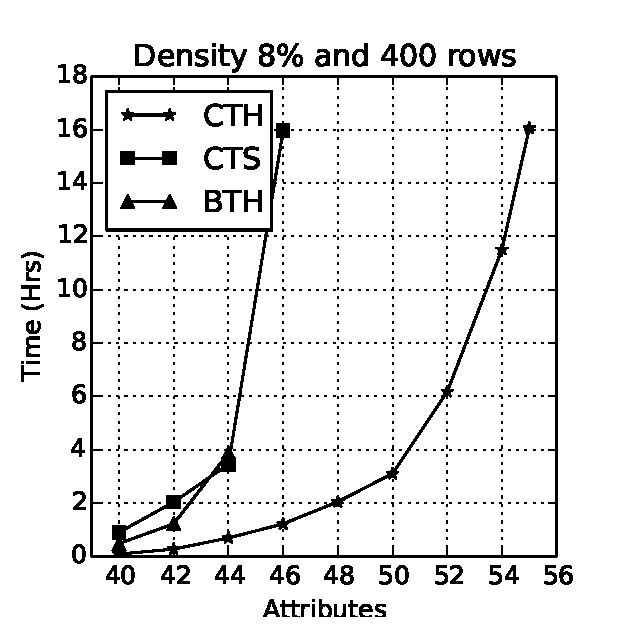
\includegraphics[width=6cm , height=6cm]{low_density.eps}
	  \caption{Total runtime for density 8\%.}
	  \label{fig:result1}
	\end{minipage}%
	\begin{minipage}{.5\textwidth}
	  \centering
	   \includegraphics[width=6cm , height=6cm]{med_density.eps}
	  \caption{Total runtime for density 33\%.}
	  \label{fig:result2}
	\end{minipage}
	\end{figure}
	
	\begin{figure}[htb]
	    \begin{center}
	       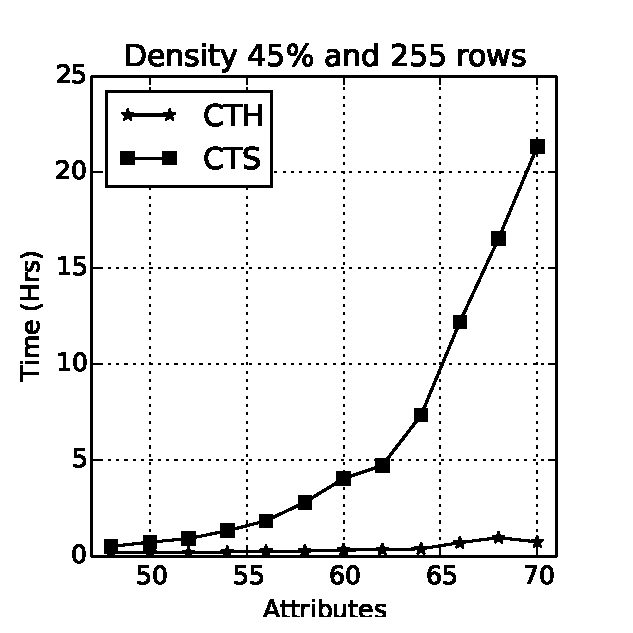
\includegraphics[height=6cm]{med48_density.eps}
	    \end{center}
	\caption{Total runtime for density 45\%.}
	\label{fig:result3}
	\end{figure}	
	
	For our experiments, 30 basic matrices of different sizes were randomly generated. 
	A random number generator was used to generate rows, which are
	filtered for the minimum and maximum number of 1's allowed. In this way the desired density was
	controlled. If accepted, the row is verified as basic against the saved rows. Basic rows 
	are saved until the desired number of rows is reached. 
	
	For the hardware platforms, we measure the runtimes including the time for the following stages: $BM$ 
	input parsing and VHDL code generation, synthesis process, and typical testor computation (with the
	hardware component running at 50MHz). The number of rows for each type of matrices is conditioned by the
	dimensions of the biggest matrix that can be synthesized at the desired running frequency.
	All experiments were performed using an Intel(R) Core(TM) i5-2400 CPU @ 3.10GHz for software executions and 
	an Atlys board, powered by a Spartan-6 LX45 FPGA device, for the hardware components.
	Figures\,\ref{fig:result1}, \,\ref{fig:result2}, and \,\ref{fig:result3} show graphics of the runtime 
	(in hours) for the three types of basic matrices. 
	
	The results of the proposed CT\_EXT hardware platform (CTH) were taken as reference for axis limits in 
	Figures\,\ref{fig:result1}, \,\ref{fig:result2}, and \,\ref{fig:result3}.
	Slowest executions of the CT\_EXT software implementation (CTS) are not shown in order to keep clarity in 
	the figures. 
	The hardware platform for BT (BTH) was not able to met the constrain of 50MHz clock frequency for some 
	matrices and running it at a lower frequency would produce longer execution time; which fall out of the limits 
	of the figures.
	
	Experiment results show that the proposed platform beats the software implementation of
	the CT\_EXT algorithm, with ratios of around one order of magnitude. However, for large 
	enough datasets this improvement could be significantly higher, as can be inferred from 
	Figure\,\ref{fig:result3}.


\subsection{A New Recursive Algorithm for Reduct Computation}
	In this subsection we present a new \textbf{R}ecursive algorithm using the \textbf{S}implified 
	\textbf{D}iscernibility \textbf{M}atrix (RSDM) for computing all the reducts in a dataset. 

\subsubsection{Concepts for RSDM}
	In this subsection we will be working with the binary representation of the simplified discernibility matrix
	(SDM). The following is a definition of super-reduct equivalent to the condition~\ref{cond_1} stated in 
	Subsection~\ref{def_reduct}.
	
	\begin{definition}\label{def:testor}
		Let $T \subseteq R$ be a subset of attributes from a dataset. We say that T is a super-reduct iff in the
		sub-matrix of SDM formed by the columns corresponding to attributes in T, there is not any zero row (row 
		having only zeros).
	\end{definition}
		
	\begin{definition}\label{def:contrib}
		Let $T \subseteq R$ and  $c_i \in R$ such that $c_i \notin T$. We say that $c_i$ contributes to T iff the
		number of zero rows, in the sub-matrix of SDM formed by the columns corresponding to attributes in 
		$T\cup\{c_i\}$, is lower than that in T.
	\end{definition}		
		
	For a fast implementation of the RSDM algorithm, columns in $SDM$ are coded as binary words with as many 
	bits as 	rows has $SDM$. The cumulative mask for an attribute $c_i$, denoted as $cm_{c_i}$, is defined as 
	the binary word representing the ith column in $SDM$. The cumulative mask for a subset of attributes $T=\lbrace
	c_{i1},c_{i2},...,c_{ik} \rbrace$ is defined	as $cm_T = cm_{c_{i1}} \vee cm_{c_{i2}} \vee ... \vee cm_{c_{ik}}$
	where $\vee$ stands for the binary OR operator. It is not hard to see that the number of 0's in $cm_T$ equals
	the number of zero rows in the sub-matrix of $SDM$ formed by the columns corresponding to attributes in T. 
	According to the definition~\ref{def:contrib}, $c_i$ contributes to $T$ iff $cm_{T\cup c_i}$ has more 1's than 
	$cm_T$. 	The incremental nature of RSDM is given by the associative property of the OR operation, such that 
	$cm_{T\cup c_i}=cm_T\vee cm_{c_i}$. Notice from this last formulation, that $c_i$ contributes to $T$ iff 
	$cm_{T\cup c_i}\neq cm_T$ since $cm_{T\cup c_i}$ cannot have less 1's than $cm_T$. It is easy to see, from 
	definition~\ref{def:testor} that $T \subseteq R$ is a super-reduct iff $cm_T=(1,...,1)$ (has a 1 in every bit).
	
	The core of the RSDM algorithm is supported by the proposition~\ref{prop3}.		
	
	\begin{proposition}\label{prop3} 
		Given $T \subseteq R$, $Z \subseteq R$ and  $c_i \in R$ such that $c_i \notin Z$ and $T \subseteq Z$. If 
		$c_i$ does not contribute to T or form a super-reduct with T, then $Z\cup\{c_i\}$ cannot be a subset of any 
		reduct.
	\end{proposition}	
	
	\begin{proof}
		As $T \subseteq Z$, $cm_T$ cannot have more 1's than $cm_Z$ by the definition of the cumulative mask.
		If $c_i$ does not contribute to $T$ then, $cm_{T \cup \lbrace c_i \rbrace}$ does not have more 1's than
		$cm_T$; and, by transitivity, $cm_{Z \cup \lbrace c_i \rbrace}$ cannot have more 1's than $cm_Z$. 
		Notice that  $\lbrace T \cup \lbrace c_i \rbrace\rbrace \subseteq \lbrace Z \cup \lbrace c_i
		\rbrace\rbrace$.
		If $T \cup \lbrace c_i \rbrace$ is a super-reduct, $\lbrace Z \cup \lbrace c_i \rbrace\rbrace$ cannot be a 
		reduct, given that it is a superset of a super-reduct; which contradicts the condition~\ref{cond_2} of the
		definition of reduct (Subsection~\ref{def_reduct})\footnote{Herein after denoted as irreducible condition} .
	\end{proof}


\subsubsection{The RSDM Algorithm}
%
	The first step in the RSDM algorithm is the sorting of the $SDM$ in order to reduce the search space. One of 
	the rows of $SDM$ having the minimum number of 1's is moved up to the first row. Then, columns are rearranged 
	so that those columns having a 1 in the first row, stay in the leftmost side of the $SDM$. A $SDM$, sorted in 
	this way, can be seen in Table~\ref{tab:SDM}. The pseudocode for RSDM is shown in algorithm~\ref{alg:RSDM}. 
	
	\renewcommand{\algorithmicrequire}{\textbf{Input:}}
	\renewcommand{\algorithmicensure}{\textbf{Output:}}
	%\begin{multicols}{2}
	\begin{algorithm}
	\caption{Recursively calculate super-reducts in $SDM$}
	\label{alg:RSDM}
	\begin{multicols}{2}
	\begin{algorithmic}[1]
	  \Require Sorted $SDM$
      \Ensure $SR$ - set of super-reducts containing all reducts
	  \State $i \Leftarrow 0$, $SR \Leftarrow \emptyset$
	  \While {$SDM(0,i) \neq 0$}\label{line:firstrow}
	  	\If {$cm_{c_i} = (1,...,1)$}\label{line:singleT}
	  		\State $SR \Leftarrow SR\cup \lbrace c_i \rbrace$
	  	\Else
	  		\State eval($\lbrace c_i \rbrace$, $cm_{c_i}$, $\lbrace c_{i+1},..., c_m\rbrace$)\label{line:eval}
	  	\EndIf
	  	\State $i \Leftarrow i+1$
	  \EndWhile
	  \item[] \item[] \item[]
	  \State eval($B$,$cm_B$,$C$)
	  \ForAll{$c \in C$} 
	  	\State $cm_{B\cup \lbrace c\rbrace}=cm_B \vee cm_c$
	  	\If {$cm_{B\cup \lbrace c\rbrace}\neq cm_B$}\label{line:contrib}
	  		\If {$cm_{B\cup \lbrace c\rbrace}=(1,...,1)$}
	  			\State $C \Leftarrow C\setminus c$\label{line:remT} 
	  			\State $SR \Leftarrow SR\cup\lbrace B\cup \lbrace c\rbrace \rbrace$
	  		\EndIf
	  	\Else
	  		\State $C \Leftarrow C\setminus c$\label{line:remNoContrib} 
	  	\EndIf
	  \EndFor
	  \ForAll{$c \in C$} 
	  	\State $C \Leftarrow C\setminus c$
	  	\State eval($B\cup \lbrace c\rbrace$,$cm_{B\cup \lbrace c\rbrace}$,$C$)\label{line:recursive} 
	  \EndFor
	\end{algorithmic}
	\end{multicols}
	\end{algorithm}
	
	
	The algorithm execution starts with the first element (column) in the sorted $SDM$ and repeats until an 
	attribute with a 0 in the first row is reached (line~\ref{line:firstrow}). Notice that for the rest of the
	candidates the first row will always be an empty row. If this single attribute is a super-reduct
	(line~\ref{line:singleT}) then it is saved in the super-reducts' set $SR$; else, the recursive evaluator 
	is called with the current attribute as the base set $B$ and the remaining attributes to its right as the 
	tail set $C$ (line~\ref{line:eval}).
	In the recursive function, every attribute in the tail is tested for contribution to the base set 
	(line~\ref{line:contrib}). The attributes are removed from the tail set for furthers evaluations, given
	that they form a super-reduct (line~\ref{line:remT}) or do not contribute to $B$
	(line~\ref{line:remNoContrib}).
	This a priori evaluation and rejection of non-contributing and testor-forming attributes constitutes the key
	gain of our proposed algorithm, and it is supported by proposition~\ref{prop3}.
	Finally, the remaining attributes in the tail set, are concatenated with $B$ and used as base set for
	subsequent recursive evaluations with the remaining $C$ as tail (line~\ref{line:recursive}).
	
	\begin{table}[!htb]
      \centering
        \caption{Sorted Simplified Discernibility Matrix}
        \begin{tabular}{ccccc}\label{tab:SDM}
            $c_0$ & $c_1$ & $c_2$ & $c_3$ & $c_4$\\
        		\hline
        		1&1&0&0&0\\
        		0&1&0&0&1\\
        		1&0&0&1&0\\
        		0&0&1&0&1\\
        		\\
        \end{tabular} 
	\end{table}	
		
	Lets take for example the simplified discernibility matrix from Table~\ref{tab:SDM}. The candidates evaluated 
	by CT\_EXT and RSDM  are shown in Table~\ref{tab:run}. Notice that while CT\_EXT evaluates 17 candidates,
	in RSDM, only 13 candidates are evaluated. Another important comment about RSDM is that the output set 
	contains all the reducts and some super-reducts that most be dismissed by checking inclusion or by any other
	way.
	
	\begin{table}[!htb]\small
		\setlength{\tabcolsep}{.1em}
		\caption{Example execution}\label{tab:run}
      	\centering
    		\begin{tabular}{|lllll|lllll|}
    		\hline
    		\multicolumn{5}{|c|}{CT\_EXT} & \multicolumn{5}{c|}{RSDM}\\
    		\hline
    		\{$ c_0$\} 	 		& \{$c_0,c_1,c_4$\}	& \{$c_0,c_3$\}		& \{$c_1,c_2,c_3$\}	& \{$c_1,c_4$\}	
    		& \{$c_0$\}			& \{$c_0,c_4$\} 		& \{$c_1,c_3$\} 		& \{$c_1,c_3,c_4$\}	&\\
    		\{$c_0,c_1$\} 		& \{$c_0,c_2$\}  	& \{$c_0,c_4$\}		& \{$c_1,c_2,c_4$\}	& 
    		& \{$c_0,c_1$\}		& \{$c_0,c_1,c_2$\} 	& \{$c_1,c_4$\}		&&\\
    		\{$c_0,c_1,c_2$\}	& \{$c_0,c_2,c_3$\}	& \{$c_1$\}			& \{$c_1,c_3$\}	  	&			
    		& \{$c_0,c_2$\} 		& \{$c_1$\}		 	& \{$c_1,c_2,c_3$\}	&&\\
    		\{$c_0,c_1,c_3$\} 	& \{$c_0,c_2,c_4$\}	& \{$c_1,c_2$\} 		& \{$c_1,c_3,c_4$\}	&			
    		& \{$c_0,c_3$\} 		& \{$c_1,c_2$\}	 	& \{$c_1,c_2,c_4$\}	&&\\
    		\hline
		\end{tabular}
	\end{table}

\subsubsection{Evaluation and Discussion}

\subsection{A New Algorithm for Reduct Computation Based on the Gap Elimination and Contribution}

	In this subsection we propose a new algorithm based on the \textbf{G}ap elimination and
	\textbf{C}ontribution, using the \textbf{S}implified \textbf{D}iscernibility \textbf{M}atrix (GCSDM), for
	computing all the reducts in a dataset. The main difference between this algorithm and CT\_EXT is the
	gap elimination; which leads to a great runtime reduction as we will show afterwards. Algorithms LEX and
	fast-BR also use the gap elimination but are based on the concept of exclusion \citep{Lias13}; which implies 
	several iterations for evaluating a candidate. GCSDM, on the other hand, is based on the concept of 
	contribution (as well as CT\_EXT) for a simpler candidate evaluation. The concept of exclusion is used in
	GCSDM, over the identified super-reducts, to verify the irreducible condition. 

\subsubsection{Concepts for GCSDM}

	The concept of gap was first introduced by \cite{Santiesteban03} for the LEX algorithm, as shown in the
	definition~\ref{def:gap}.
	
	\begin{definition}\label{def:gap}
		Let $L \subseteq R$ be a subset of attributes from a dataset, such that $L = \lbrace c_{j_0},...,c_{j_s}
		\rbrace$ and $c_{j_0}<\cdots <c_{j_s}$. We denote the attribute $c_p \in L$ gap of L, where $j_0 \leq p \leq
		j_s$ such that $p=\mathrm{max}(j_q | c_{j_q},c_{j_{q+1}} \in L \wedge j_{q+1} \neq j_q)$.
	\end{definition}
	
	In other words, the gap is the attribute in $L$ with the highest index such that its consecutive attribute in 
	$L$ is not its consecutive attribute in $SDM$.
	
	\begin{table}[!htb]
      \centering
        \caption{Sorted Simplified Discernibility Matrix}
        \begin{tabular}{ccccccc}\label{tab:SDM1}
            $c_0$ & $c_1$ & $c_2$ & $c_3$ & $c_4$ & $c_5$ & $c_6$\\
        		\hline
        		1&0&0&0&0&0&0\\
        		0&1&0&1&0&0&0\\
        		0&0&0&0&0&0&1\\
        		0&0&1&0&1&0&0\\
        		0&0&0&0&0&1&0\\
        \end{tabular} 
	\end{table}
	
	Lets take for example the simplified discernibility matrix from Table~\ref{tab:SDM1}:
	$$\begin{array}{ll}
	\lbrace c_0,c_1,c_2,c_3\rbrace 		& \mathrm{there~is~no~gap}\\
	\lbrace c_0,c_1,c_2,c_5,c_6\rbrace 	& \mathrm{the~gap~is~} c_2\\
	\lbrace c_0,c_1,c_2,c_4,c_6\rbrace 	& \mathrm{the~gap~is~} c_4\\
	\lbrace c_0,c_1,c_4,c_5,c_6\rbrace 	& \mathrm{the~gap~is~} c_1
	\end{array}$$
	
	
	The gap elimination is supported by the proposition~\ref{prop:gap}. In order to clarify the basis of the gap
	elimination we exemplify the lexicographical traversing order with a $SDM$ of three attributes:
	
	\{$c_0$\}, \{$c_0,c_1$\}, \{$c_0,c_1,c_2$\}, \{$c_0,c_2$\}, \{$c_1$\}, \{$c_1,c_2$\}, \{$c_2$\}
		
	\begin{proposition}\label{prop:gap} 
		Let $L \subseteq R$ be a reduct, such that $L = \lbrace c_{j_0},...,c_{j_s}\rbrace$, $c_{j_0}<\cdots <c_{j_s}$
		and $c_{j_s}$ is the last attribute in SDM. If there is a gap $c_p$ in L, being $L' = \lbrace
		c_{j_0},...,c_{j_k},c_{p+1}\rbrace$, $j_0<\cdots <j_k<=p-1$; then, there is no any attribute subset 
		between L and $L'$ (following the lexicographical order) being a reduct.
	\end{proposition}	
	
	\begin{proof}
		Lets denote $L$ as $\mu+\delta$, where $\delta= \lbrace c_{j_q}, c_{j_q+1},...,c_{j_s}\rbrace$, $j_q>p+1$
		and $\mu = \lbrace c_{j_0},...,c_{j_k},c_{j_p}\rbrace$; such that attributes in $\delta$ are consecutive 
		in $SDM$. Every attribute subset between L and $L'$ (following the	lexicographical order) can be 
		denoted as $\lambda=\mu+\nu$, where $\nu \subset \delta$. Thus, every $\lambda$ between L and $L'$ is a
		proper subset of $L$. Given that L is a reduct, a proper subset of L cannot be a reduct according to the 
		irreducible condition of reducts. 
	\end{proof}
	
	From the proposition~\ref{prop:gap} we have the following corollary; which is relevant to GCSDM in order to
	avoid more unnecessary evaluations.
	
	\begin{corollary}\label{coro:gap} 
		Let $L \subseteq R$ be not a super-reduct, such that $L = \lbrace c_{j_0},...,c_{j_s}\rbrace$, 
		$c_{j_0}<...<c_{j_s}$ and $c_{j_s}$ is the last attribute in SDM. If there is a gap $c_p$ in L, being 
		$L' = \lbrace c_{j_0},...,c_{j_k},c_{p+1}\rbrace$, $j_0<...<j_k<=p-1$; then, there is no any attribute 
		subset between L and $L'$ (following the lexicographical order) being a reduct.
	\end{corollary}
	
	In Table~\ref{tab:patial} we show a partial execution of CT\_EXT over the $SDM$ from Table~\ref{tab:SDM1} to 
	illustrate the principle of the gap elimination. The first 17 evaluated candidates, out of 41, are presented 
	along with their evaluation. For this particular case, GCSDM requires the evaluation of only 23 candidates 
	for a runtime reduction above the 40\%. Candidates of iterations 7 and 12 are reducts which include the last
	attribute in $SDM$ ($c_6$). Candidates of iterations 8, 13, 14, 15 and 16 are proper subsets of reducts, as
	indicated by the proposition~\ref{prop:gap}, and cannot be a reduct. Thus; the evaluation of these candidates,
	with a gray background in Table~\ref{tab:patial}, is unnecessary. 
	
	\begin{table}[!htb]
		\caption{Partial execution. The evaluation of a candidate subset is labelled as C - the added attribute 
				 contributes, NC - the added attribute does not contribute, R - the candidate is a reduct, or
				 NSR - the last attribute is reached and the candidate is not a super-reduct.}\label{tab:patial}
      	\centering
    		\begin{tabular}{|c|lc|c|lc|}
    		\hline
    		Iter & \multicolumn{1}{c}{Candidate} & \multicolumn{1}{c|}{Evaluation}
    		& Iter & \multicolumn{1}{c}{Candidate} & \multicolumn{1}{c|}{Evaluation}\\
    		\hline
    		~1 & \{$c_0$\} 	 				& C		& 10 & \{$c_0,c_1,c_4$\} 			& C \\	
    		~2 & \{$c_0,c_1$\}				& C 		& 11 & \{$c_0,c_1,c_4,c_5$\}		& C \\
    		~3 & \{$c_0,c_1,c_2$\} 			& C  	& 12 & \{$c_0,c_1,c_4,c_5,c_6$\}*	& R \\
    		~4 & \{$c_0,c_1,c_2,c_3$\}		& NC 	& 13 & \cellcolor[gray]{0.9}\{$c_0,c_1,c_4,c_6$\}	& NSR\\
    		~5 & \{$c_0,c_1,c_2,c_4$\}		& NC 	& 14 & \cellcolor[gray]{0.9}\{$c_0,c_1,c_5$\}		& C \\
    		~6 & \{$c_0,c_1,c_2,c_5$\} 		& C		& 15 & \cellcolor[gray]{0.9}\{$c_0,c_1,c_5,c_6$\} & NSR \\
    		~7 & \{$c_0,c_1,c_2,c_5,c_6$\}*	& R  	& 16 & \cellcolor[gray]{0.9}\{$c_0,c_1,c_6$\}	& NSR \\
    		~8 & \cellcolor[gray]{0.9}\{$c_0,c_1,c_2,c_6$\} 		& NSR 	& 17 & \{$c_0,c_2$\}			& C \\
    		~9 & \{$c_0,c_1,c_3$\}			& NC 	&$\cdots$& ~~~~$\cdots$		& $\cdots$\\
    		\hline
		\end{tabular}
	\end{table}
	
	In order to determine whether a super-reduct is a reduct (verifying the irreducible condition) the
	exclusion mask, introduced by \cite{Lias09}, plays a fundamental role. 
	
	\begin{definition}\label{def:exclusion}
		Let $L \subseteq R$ be a subset of attributes from a dataset. We call exclusion mask of L, denoted as 
		$em_L$, to the binary word in which the ith bit is 1 if the ith row in $SDM$ has only 1 in a single 
		column of those columns corresponding to attributes in L, and it is 0 otherwise.
	\end{definition}
	
	For instance, from the $SDM$ in Table~\ref{tab:SDM1} we have:
	$$\begin{array}{lcc}
	  em_{\lbrace c_0,c_1,c_2\rbrace}         &=& (1,1,0,1,0)\\
	  em_{\lbrace c_0,c_1,c_2,c_3\rbrace}     &=& (1,0,0,1,0)\\
	  em_{\lbrace c_0,c_1,c_2,c_3,c_4\rbrace} &=& (1,0,0,0,0)
	\end{array}$$
	
	\cite{Lias13} proposed the following to support the cumulative computation of the exclusion mask.
	
	\begin{proposition}\label{prop:cumul} 
		Let $L \subseteq R$ be a subset of attributes from a dataset and $c \notin L$ an attribute of $SDM$.
		The exclusion mask of $L \cup \lbrace c\rbrace$ is calculated as follows:
		$$em_{L \cup \lbrace c\rbrace}=(em_L \wedge \neg cm_c) \vee (\neg cm_L \wedge cm_c)$$
		where $cm$ refers to the cumulative mask.
	\end{proposition}
	
	Finally, they stated and proved the following proposition.
	
	\begin{proposition}\label{prop:exclude} 
		Let $L \subseteq R$ be a subset of attributes from a dataset and $c \notin L$ an attribute of $SDM$.
		If $\exists c_i \in L$ such that $em_{L \cup \lbrace c\rbrace} \wedge cm_{c_i}=(0,...,0)$. Then, c
		does not form a reduct with L.
	\end{proposition}
	
	
\subsubsection{The GCSDM Algorithm}	

	The first step in the GCSDM algorithm is the sorting of the $SDM$ in the same way as we did for RSDM. 
	The pseudocode for GCSDM is shown in algorithm~\ref{alg:GCSDM}. Unlike RSDM, this algorithm returns
	only the set of all reducts. In this sense; it has not advantage over RSDM or CT\_EXT, since they all can 
	use the same procedure to dismiss supersets of reducts.
	
	We start with an empty base subset $B$ and the position of the first attribute in $c$\footnote{Here we 
	abuse of notation by using $c$ for both an attribute and a number denoting its position in $SDM$}. Then
	we assign a null vector to the cumulative mask ($cm_B$) for $B=\emptyset$ or retrieve its calculated value
	for	$B\neq \emptyset$ (lines~\ref{line:emptyB}-\ref{line:notEmpty}). $CM$ stores the calculated cumulative 
	masks, indexed by the last attribute in $B$.	The function getLast$(B)$ returns the last attribute in $B$
	or its position as the case may be. In the line~\ref{line:updateCM} we update the cumulative mask and in
	the line~\ref{line:contrib} we evaluate the contribution of $c$ to $B$. The cumulative mask of an 
	attribute $cm_c$ has the same meaning as in RSDM. If the current attribute $c$ contributes, we evaluate
	the super-reduct condition on $B\cup \lbrace c\rbrace$ (line~\ref{line:superReduct}). For super-reducts,
	we use the proposition~\ref{prop:cumul} to compute the exclusion mask $em_{B\cup \lbrace c\rbrace}$ 
	(lines~\ref{line:em}-\ref{line:emEnd}) and verify the irreducible condition (lines~\ref{line:reduct}-
	\ref{line:reductEnd}), by means of the proposition~\ref{prop:exclude}. At this point, the candidate 
	evaluation is finished.
	
	From line~\ref{line:cg} to the end, the next candidate subset ($B\cup \lbrace c\rbrace$) is generated. 
	The value LastAttribute holds the position of the last attribute in $SDM$. If the last attribute is
	reached, given that the current candidate is a reduct or it is not a super-reduct, we eliminate the gap
	(lines~\ref{line:gap}-\ref{line:gapEnd}). If the last attribute is reached but the current candidate is 
	a super-reduct, the last attribute in $B$ is removed (line~\ref{line:remLast}). If the last attribute is 
	not reached yet, there are two possibilities. The current candidate is a super-reduct or the current
	attribute $c$ does not contributes to $B$; then we most replace $c$ by the next attribute in $SDM$
	(line~\ref{line:replaceC}). The attribute $c$ contributes to $B$ and the current candidate is not a 
	super-reduct; then the current attribute is added to $B$ (line~\ref{line:add1}) and the next attribute in 
	$SDM$ is loaded to $c$ (line~\ref{line:add1End}). The algorithm finishes once the column corresponding 
	to the first attribute in the current candidate has a 0 in the first row.
	
	\begin{algorithm}
	\caption{GCSDM algorithm for computing all reducts}
	\label{alg:GCSDM}
	\begin{algorithmic}[1]
	  \Require Sorted $SDM$
      \Ensure $RR$ - the complete set of reducts
	  \State $B \Leftarrow \emptyset$, $RR \Leftarrow \emptyset$, $c \Leftarrow 0$
	  \While {\textbf{not} done}
	  \State $reduct \Leftarrow \mathrm{False}$, $superReduct \Leftarrow \mathrm{False}$, 
	  		 $contributes \Leftarrow \mathrm{False}$
	  	\If {$B = \emptyset$}\label{line:emptyB}
	  		\State $cm_B \Leftarrow (0,...,0)$
	  	\Else
	  		\State $cm_B \Leftarrow CM[\mathrm{getLast}(B)]$\label{line:notEmpty}
	  	\EndIf
	  	\State $cm_{B\cup \lbrace c\rbrace} \Leftarrow cm_B \vee cm_c$\label{line:updateCM}
	  	\State $CM[c] \Leftarrow cm_{B\cup \lbrace c\rbrace}$
	  	\If {$cm_{B\cup \lbrace c\rbrace}\neq cm_B$}\label{line:contrib}
	  		\State $contributes \Leftarrow \mathrm{True}$
	  		\If {$cm_{B\cup \lbrace c\rbrace}=(1,...,1)$}\label{line:superReduct}
	  			\State $superReduct \Leftarrow \mathrm{True}$
	  			\State $em_{B\cup \lbrace c\rbrace} \Leftarrow (0,...,0)$, $cm \Leftarrow (0,...,0)$
	  			\ForAll{$x \in B\cup \lbrace c\rbrace$} \label{line:em}
	  				\State $em_{B\cup \lbrace c\rbrace} \Leftarrow (em_{B\cup \lbrace c\rbrace}\wedge \neg 
	  						cm_x) \vee (\neg cm \wedge cm_x)$
	  				\State $cm \Leftarrow CM[x]$\label{line:emEnd}
	  			\EndFor
	  			\State $reduct \Leftarrow \mathrm{True}$\label{line:reduct}
	  			\ForAll{$x \in B$} 
	  				\If {$em_{B\cup \lbrace c\rbrace}\wedge cm_x=(0,...,0)$}
	  					\State $reduct \Leftarrow \mathrm{False}$
	  					\State \textbf{break}\label{line:reductEnd}
	  				\EndIf
	  			\EndFor
	  		\EndIf
	  	\EndIf
	  	\If {$c=$LastAttribute} \Comment{Reached the last column of the binary $SDM$}\label{line:cg}
	  		\If {$reduct$ \textbf{or} \textbf{not} $superReduct$} \Comment{Eliminate existing 
	  																			gap}\label{line:gap}
	  			\State $last \Leftarrow c$
	  			\While {$\mathrm{getLast}(B)=(last-1)$}
	  				\State $last \Leftarrow \mathrm{getLast}(B)$
	  				\State $B \Leftarrow B\setminus last$
	  				\If {$\vert B \vert =1$}
	  					\State \textbf{break}\label{line:gapEnd}
	  				\EndIf
	  			\EndWhile
	  		\EndIf
	  		\State $c \Leftarrow  \mathrm{getLast}(B)+1$
	  		\State $B \Leftarrow B\setminus \mathrm{getLast}(B)$\label{line:remLast}
	  	\Else
	  		\If {\textbf{not} $contributes$ \textbf{or} $superReduct$}
	  			\State $c \Leftarrow c+1$\label{line:replaceC}
	  		 \EndIf
	  		 \If {$contributes$ \textbf{and} \textbf{not} $superReduct$}
	  			\State $B \Leftarrow B\cup c$\label{line:add1}
	  			\State $c \Leftarrow c+1$\label{line:add1End}
	  		 \EndIf
	  	\EndIf
	  	\If {$B = \emptyset$ \textbf{and} $cm_c[0] = 0$} \Comment{First attribute has a 0 in the first 
	  																			row}\label{line:done}
	  		\State $done \Leftarrow \mathrm{True}$
	  	\EndIf
	  \EndWhile 
	\end{algorithmic}
	\end{algorithm}
	
	In Table~\ref{tab:sample_GCSDM} we show a sample execution of GCSDM over the $SDM$ from Table~\ref{tab:SDM1}.
	The columns labelled C, SR and R stands for the candidate evaluation results on \textbf{C}ontribution, 
	\textbf{S}uper-\textbf{R}educt and \textbf{R}educt conditions, respectively. Notice that the gap elimination 
	occurs after candidates of iterations 7, 11, 16, 23 (reducts) and 19 (not super-reduct).
	
	\begin{table}[!htb]
		\caption{Sample Execution of GCSDM.}\label{tab:sample_GCSDM}
      	\centering
    		\begin{tabular}{|c|l|c|l|c|c|c|l|}
    		\hline
    		Iter & \multicolumn{1}{c|}{$B$} & $c$ & \multicolumn{1}{c|}{$B\cup \lbrace c\rbrace$} 
    		& C & SR & R & \multicolumn{1}{c|}{Comments}\\
    		\hline
    		~1 & \{\} 					& 0 & \{$c_0$\} 					& True & False &   & Add a new attribute.\\
    		~2 & \{$c_0$\} 				& 1 & \{$c_0,c_1$\}				& True & False &   & Add a new attribute.\\
    		~3 & \{$c_0,c_1$\} 			& 2 & \{$c_0,c_1,c_2$\}			& True & False &   & Add a new attribute.\\
    		~4 & \{$c_0,c_1,c_2$\} 		& 3 & \{$c_0,c_1,c_2,c_3$\}		& False &   &   & Remove $c_3$ (proposition~\ref{prop3}).\\
    		~5 & \{$c_0,c_1,c_2$\} 		& 4 & \{$c_0,c_1,c_2,c_4$\}		& False &   &   & Remove $c_4$ (proposition~\ref{prop3}).\\
    		~6 & \{$c_0,c_1,c_2$\}		& 5 & \{$c_0,c_1,c_2,c_5$\}		& True & False &   & Add a new attribute.\\
    		~7 & \{$c_0,c_1,c_2,c_5$\}	& 6 & \{$c_0,c_1,c_2,c_5,c_6$\} 	& True & True & True & Eliminate the gap ($c_2$).\\
    		~8 & \{$c_0,c_1$\} 			& 3 & \{$c_0,c_1,c_3$\}			& False &   &   & Remove $c_3$ (proposition~\ref{prop3}).\\
    		~9 & \{$c_0,c_1$\}			& 4 & \{$c_0,c_1,c_4$\}			& True & False &   & Add a new attribute.\\
    		10 & \{$c_0,c_1,c_4$\}		& 5 & \{$c_0,c_1,c_4,c_5$\}		& True & False &   & Add a new attribute.\\
    		11 & \{$c_0,c_1,c_4,c_5$\}	& 6 & \{$c_0,c_1,c_4,c_5,c_6$\} 	& True & True & True & Eliminate the gap ($c_1$).\\
    		12 & \{$c_0$\} 				& 2 & \{$c_0,c_2$\}				& True & False &   & Add a new attribute.\\
    		13 & \{$c_0,c_2$\} 			& 3 & \{$c_0,c_2,c_3$\}			& True & False &   & Add a new attribute.\\
    		14 & \{$c_0,c_2,c_3$\} 		& 4 & \{$c_0,c_2,c_3,c_4$\}		& False &   &   & Remove $c_4$ (proposition~\ref{prop3}).\\
    		15 & \{$c_0,c_2,c_3$\}		& 5 & \{$c_0,c_2,c_3,c_5$\}		& True & False &   & Add a new attribute.\\
    		16 & \{$c_0,c_2,c_3,c_5$\}	& 6 & \{$c_0,c_2,c_3,c_5,c_6$\} 	& True & True & True & Eliminate the gap ($c_3$).\\
    		17 & \{$c_0,c_2$\} 			& 4 & \{$c_0,c_2,c_4$\}			& False &   &   & Remove $c_4$ (proposition~\ref{prop3}).\\
    		18 & \{$c_0,c_2$\}			& 5 & \{$c_0,c_2,c_5$\}			& True & False &   & Add a new attribute.\\
    		19 & \{$c_0,c_2,c_5$\}		& 6 & \{$c_0,c_2,c_5,c_6$\}		& True & False &   & Eliminate the gap ($c_2$).\\
    		20 & \{$c_0$\} 				& 3 & \{$c_0,c_3$\}				& True & False &   & Add a new attribute.\\    		
    		21 & \{$c_0,c_3$\}			& 4 & \{$c_0,c_3,c_4$\}			& True & False &   & Add a new attribute.\\
    		22 & \{$c_0,c_3,c_4$\}		& 5 & \{$c_0,c_3,c_4,c_5$\}		& True & False &   & Add a new attribute.\\
    		23 & \{$c_0,c_3,c_4,c_5$\}	& 6 & \{$c_0,c_3,c_4,c_5,c_6$\} 	& True & True & True & Eliminate the gap ($c_0$).\\
    		\hline
    		24 & \{\} 					& 1 & \{$c_1$\} 					& 
    		\multicolumn{4}{l|}{\scriptsize Algorithm finishes because $c_1$ has a 0 in the first row of $SDM$ (line~\ref{line:done})}\\
    		\hline
		\end{tabular}
	\end{table}
	
	\cite{Alba14} pointed out that CT\_EXT has a surprisingly low performance over identity matrices. 
	In fact, CT\_EXT traverses the complete power set of attribute combinations. The introduction of
	the gap elimination solves this drawback in such a way that a minimum number of candidate 
	verifications is required for this kind of matrices.

\subsubsection{Evaluation and Discussion}

	In order to evaluate the performance of GCSDM, we present here a comparative analysis of different
	algorithms over synthetically generated simplified discernibility matrices. For this experiment we
	selected CT\_EXT and fastBR in addition to our two proposals. These algorithms are reported in the 
	literature as the fastest algorithms for typical testor computation. Algorithms for computing all
	reducts such as RGonCRS \citep{WangP07} and that proposed in \citep{Starzyk00} were not included
	since they showed a lower performance in our preliminary experiments. 
	
	The experimental units for this experiments are 57 randomly generated $SDM$. Our independent 
	variables are the density of 1's in the $SDM$ and the standard deviation of density of 1's in rows
	of $SDM$. The distribution of values for these variables is shown in Figures~\ref{fig:density} 
	and~\ref{fig:std} respectively. The dependent variable is the fastest algorithm; whose levels are:
	CT\_EXT, fastBR, RSDM and GCSDM. The treatments are the selected algorithms; which are applied
	all to every experimental unit. Each combination is executed three times and the runtime is 
	estimated by the fastest execution. This process ensures us a 95\% confidence interval according
	to \cite{Haveraaen01}. The execution order was randomized to control the runtime bias due to the
	operating system load. All experiments were run on a G1620 Intel processor at 2.7GHz with 2GB
	in RAM over a GNU/Linux operating system.
	
	\begin{figure}[htb]
	\begin{minipage}{.5\textwidth}
	    \begin{center}
	       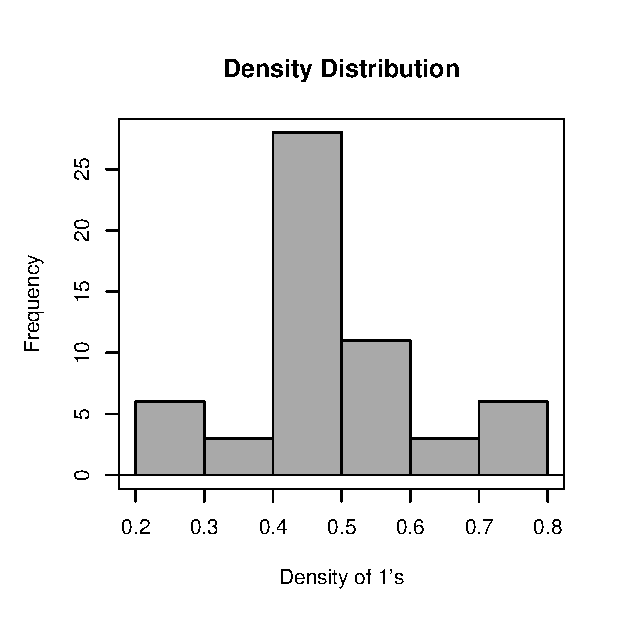
\includegraphics[height=8cm]{density_freq.eps}
	    \end{center}
	\caption{Distribution of densities in $SDM$ under study.}
	\label{fig:density}
	~
	\end{minipage}%
	\begin{minipage}{.5\textwidth}
	    \begin{center}
	       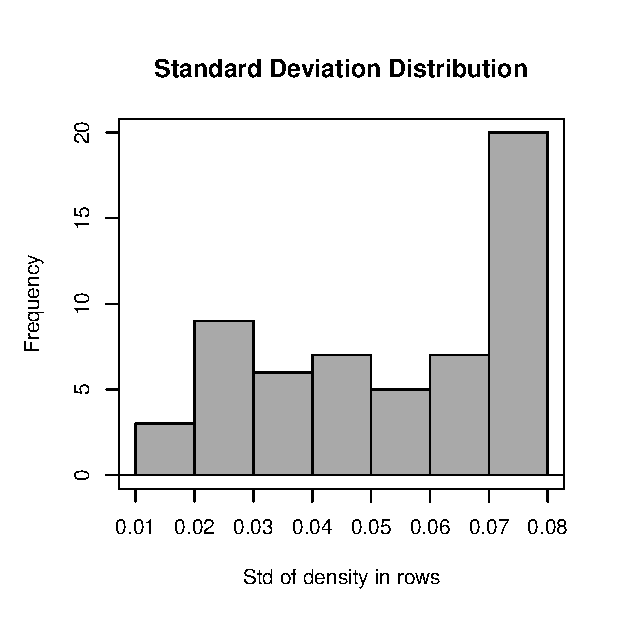
\includegraphics[height=8cm]{std_freq.eps}
	    \end{center}
	\caption{Distribution of standard deviation of density in rows for all $SDM$ under study.}
	\label{fig:std}
	\end{minipage}	
	\end{figure}		
	
	In order to obtain the desired density and standard deviation of density in rows, we used the 
	matrix generator described in subsection~\ref{subsect:CTEXT_eval}. We control the maximum and
	minimum number of 1's in a randomly generated row. In this way, the desired density is computed
	as the mean number of 1's in a row, divided by the number of attributes (columns). Keeping 
	constant this central value, we can modify at the same time the maximum and minimum number of
	allowed 1's in a row to control the standard deviation. For each desired pair of values (density 
	and standard deviation), three different matrices were generated.
	
	Figure~\ref{fig:scattDensity} shows a scatter plot of the execution runtime as a function of 
	the density of 1's in the $SDM$. The execution runtime is taken from the fastest algorithm for 
	each case. The dots are grouped by the best performing (fastest)	algorithm for that particular 
	matrix as shown in the legend of the figure. There can be identified three distinct groups of 
	matrices by its density:
	\begin{itemize}
	\item Low density matrices: density $<$ 0.3.
	\item Medium density matrices: 0.3 $<$ density $<$ 0.7.
	\item High density matrices: density $>$ 0.7.
	\end{itemize}
	The best performing algorithm for all low density matrices is GCSDM, fastBR was the fastest for
	all medium density matrices and RSDM outperforms the other algorithms in most of the high
	density matrices. The fact that high density $SDM$ does not constitute a complex computational
	task for reduct computation is clearly visible in Figure~\ref{fig:scattDensity}. Notice that
	CT\_EXT was never the best performing algorithm while fastBR was the fastest in the greater number
	of matrices.
		
	\begin{figure}[htb]
	\begin{minipage}{.48\textwidth}
	    \begin{center}
	       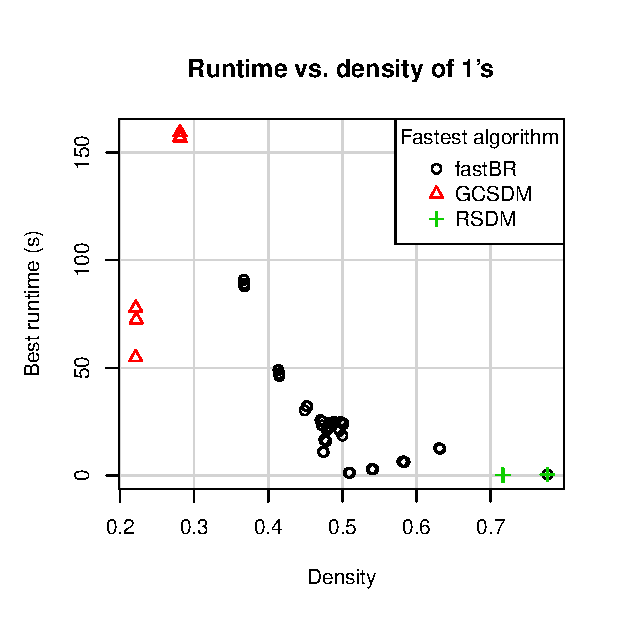
\includegraphics[height=8cm]{scatter_density.eps}
	    \end{center}
	\caption{Best performing algorithm runtime vs. density of 1's for all $SDM$ under study.}
	\label{fig:scattDensity}
	\end{minipage}%
	~
	\begin{minipage}{.48\textwidth}
	    \begin{center}
	       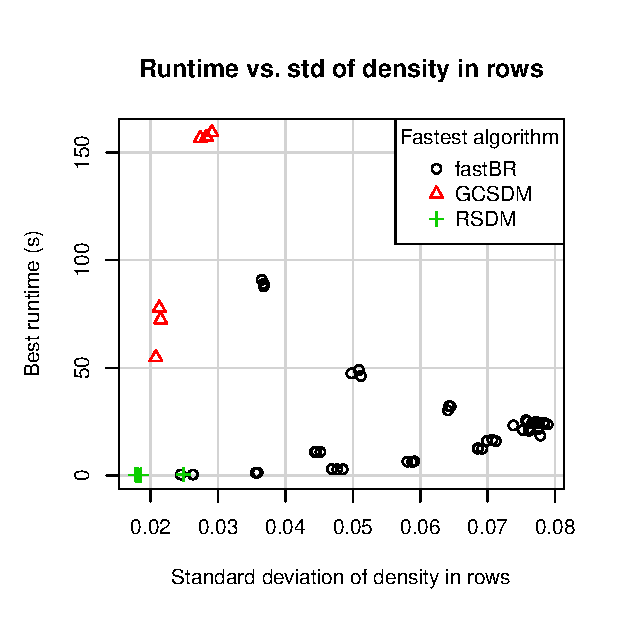
\includegraphics[height=8cm]{scatter_std.eps}
	    \end{center}
	\caption{Best performing algorithm runtime vs. standard deviation of density in rows for 
			 all $SDM$ under study.}
	\label{fig:scattStd}
	\end{minipage}	
	\end{figure}	
	
	Since all matrices for this experiment have the same dimensions, we can say that low density
	matrices showed a relatively high complexity. For this reason, the apparent fact that GCSDM outperforms 
	the other algorithms for this kind of matrices, deserves special attention. On the other hand, result 
	of RSDM on high density matrices presents a lesser importance. Figure~\ref{fig:scattDensity} shows a trend
	to the reduction of the computational complexity of reduct computation, regarding the increase of the
	density in the $SDM$.
	
	Figure~\ref{fig:scattStd} shows a scatter plot of the execution runtime as a function of 
	the standard deviation of the density of 1's in the rows of the $SDM$. As can be seen, there is no
	clear relationship between the runtime or the fastest algorithm and the standard deviation of density.
	Notice (combining information from Figures~\ref{fig:scattDensity} and~\ref{fig:scattStd}) that both, 
	low and high density matrices are related to low values of the standard deviation. In fact, it impossible
	to increase the standard deviation in the extremes values of density without affecting the mean
	number of 1's in a row.
	
	Figure~\ref{fig:TimeReducts} shows a scatter plot of the execution runtime as a function of the 
	number of reducts in the $SDM$. There can be seen a positive correlation between these two variables.
	This trend is natural since we all know that the time complexity is at least as high as the space 
	complexity which exceeds the size of the solution. For low density matrices we can see a runtime cost
	beyond the trend for the rest of matrices. For high density matrices, there can be seen a low number
	of reducts which partially explains their low runtime. 
	
	\begin{figure}[htb]
	\begin{minipage}{.48\textwidth}
	    \begin{center}
	       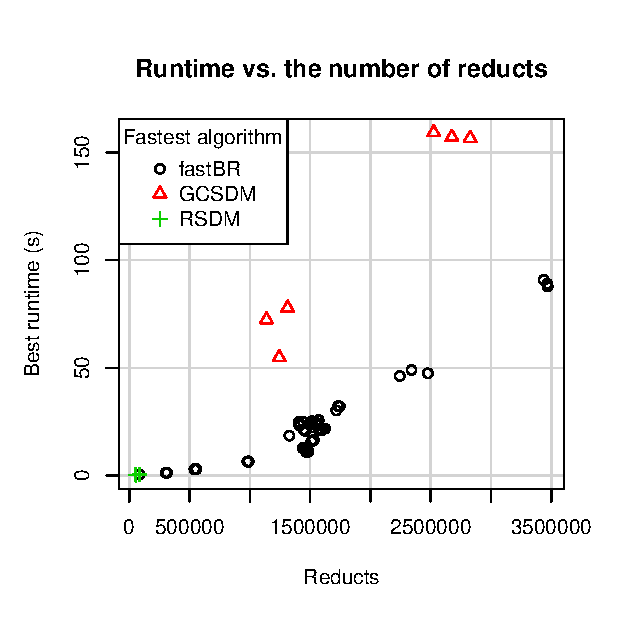
\includegraphics[height=8cm]{runtimeReducts.eps}
	    \end{center}
	\caption{Best performing algorithm runtime vs. the number of reducts.}
	\label{fig:TimeReducts}
	\end{minipage}%
	~
	\begin{minipage}{.48\textwidth}
	    \begin{center}
	       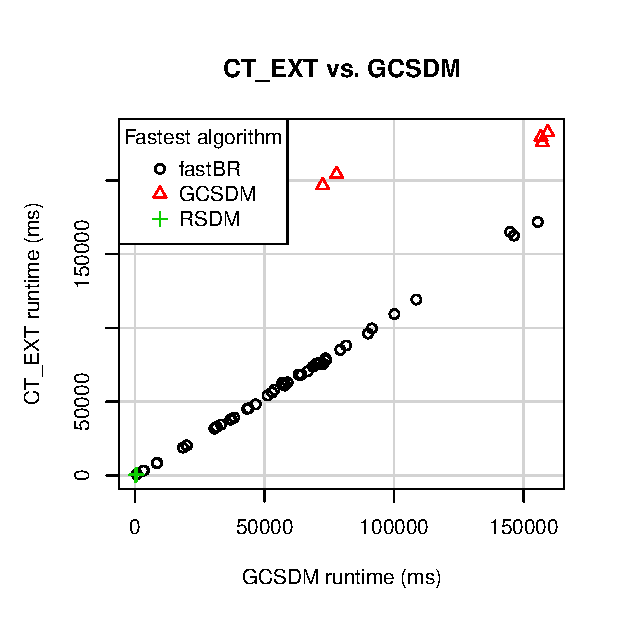
\includegraphics[height=8cm]{scatter_CTvsGAP.eps}
	    \end{center}
	\caption{CT\_EXT runtime vs. GCSDM runtime.}
	\label{fig:CTvsGAP}
	~
	\end{minipage}	
	\end{figure}		
	
	Figure~\ref{fig:CTvsGAP} shows a scatter plot of the runtime of CT\_EXT vs. GCSDM for the $SDM$ used in
	this experiments. Although GCSDM outperforms CT\_EXT in most cases, we can see that there is a specially
	high runtime gain for low density matrices. Based on the evidence of Figure~\ref{fig:CTvsGAP}, we 
	proposed a one-sided t-test to evaluate the overall performance of GCSDM over CT\_EXT. We suppose that
	our sample of 57 $SDM$ is a random sample representing the universe of $SDM$ and state the following
	\textbf{null hypothesis}: \emph{there is no difference between the GCSDM and CT\_EXT runtime}. As 
	\textbf{alternative hypothesis} we have: \emph{the runtime of CT\_EXT is greater than the runtime of GCSDM}.
	The output from R\footnote{http://www.r-project.org} software supports the alternative hypothesis beyond
	a 95\% confidence interval. Indeed, the p-value suggest that the probability of obtaining an experimental
	result like that shown in Figure~\ref{fig:CTvsGAP}, given that the null hypothesis is true, is only 
	0.0008428.
	
	\begin{quote}
		\qquad{}	Paired one-sided t-test\\

		data:  CT\_EXT runtime and GCSDM runtime\\
		t = 3.3, df = 56, p-value = 0.0008428\\
		alternative hypothesis: true difference in means is greater than 0\\
		95 percent confidence interval:\\
		 6976.147ms  \qquad{}  Inf\\
		sample estimates:\\
		mean of the differences \\
		 \qquad{}    14145.54ms
	\end{quote}

\newpage 
\section{Conclusions}
	This PhD. research proposal is focused on the problem of computing all the reducts and its related problem of
	computing shortest reducts of an information system. These are problems with exponential complexity which are
	actively studied. The theoretical bases were introduced to provide a unique nomenclature for the document and
	ensure that it is self contained. We present a revision of the related work to show the most relevant approach
	to the problem solution as well as need of new research in this area. Then, the methodology that will guide 
	our future research is presented.
	
	As preliminary results, we presented two new hardware architectures for computing typical testors and two new
	algorithms for reduct computation. Our first work is a modified hardware platform for computing typical 
	testors and was published in the memories of a relevant international conference on reconfigurable computing.
	Our second result is a new hardware architecture for computing typical testors and it is currently under the
	second revision to be published on a journal. Our two proposed algorithm for computing all reducts were faster
	than existing algorithms for some kinds of datasets.
	
	Finally, based on our preliminary results, we conclude that our objectives are reachable, in the scheduled
	time, following 	the proposed methodology.
	
%-------------------------------------------------------------------------------
% Bibliography
%-------------------------------------------------------------------------------
\newpage 
\bibliography{mybib}{}
\bibliographystyle{authordate1}
\end{document}
